% Autor: Alfredo Sánchez Alberca (asalber@ceu.es)
\section{Variables Aleatorias}

\mode<presentation>{
%---------------------------------------------------------------------slide----
\begin{frame}
\frametitle{Variables aleatorias discretas}
\tableofcontents[sectionstyle=show/hide,hideothersubsections]
\end{frame}
}


%---------------------------------------------------------------------slide----
\begin{frame}
\frametitle{Variables aleatorias}
Cuando seleccionamos una muestra al azar de una población estamos realizando un experimento aleatorio y cualquier variable estadística medida a partir de la muestra será una variable aleatoria porque sus valores dependerán del azar. 

\begin{definicion}[Variable Aleatoria] 
Una \emph{variable aleatoria} $X$ es una función que asocia un número real a cada elemento del espacio muestral de un experimento aleatorio. 
\[ 
	X:\Omega \rightarrow \mathbb{R} 
\]

Al conjunto de posibles valores que puede tomar la variable aleatoria se le llama \emph{rango} o \emph{recorrido} de la variable, y se representa por $\mbox{Ran}(X)$.
\end{definicion}

En el fondo, una variable aleatoria es una variable cuyos valores provienen de la realización de un experimento aleatorio, y por tanto, tendrá asociada una determinada distribución de probabilidad.

\textbf{Ejemplo}. La variable $X$ que mide el resultado del lanzamiento de un dado es una variable aleatoria y su rango es 
\[
	\mbox{Ran}(X)=\{1,2,3,4,5,6\}
\]

\note{
Con este tema entramos de lleno en la inferencia estadística, que tiene por objeto construir modelos probabilísticos que
expliquen el comportamiento de las variables en las poblaciones. Estas variables se llaman variables aleatorias porque al medirlas en
la muestra obtenida al azar de la población, sus valores provienen de realizar un experimento aleatorio.  

\begin{definicion}[Variable Aleatoria] 
Una \emph{variable aleatoria} $X$ es una función que asocia un número real a cada elemento del
espacio muestral de un experimento aleatorio. \[ X:E\rightarrow \mathbb{R} \]

Al conjunto de posibles valores que puede tomar la variable aleatoria se le llama \emph{rango} o \emph{recorrido} de la variable.
\end{definicion}

Como los valores de una variable aleatoria provienen de la realización de un experimento aleatorio, 
tendrá asociada una determinada distribución de probabilidad. Nuestro objetivo es conocer lo mejor posible esa distribución de probabilidad
pero debemos recordar que cuando estudiemos una determinada variable,
normalmente no conoceremos con exactitud cómo se distribuyen sus valores en la población, ya que no podremos medir a todos los invididuos de
la misma. Por tanto, los modelos de distribución de probabilidad que utilizaremos para describir el comportamiento de las variables en las
poblaciones serán modelos aproximados. 

Un ejemplo de variable aleatoria es la que mide el resultado del lanzamiento de un dado.
}
\end{frame}


%---------------------------------------------------------------------slide----
\begin{frame}
\frametitle{Tipos de variables aleatorias}
Las variables aleatorias se clasifican en dos tipos:
\begin{description}
\item[Discretas (VAD):] Toman valores aislados y su rango es numerable.\\
Ejemplo. Número de hijos, número de cigarrillos, número de asignaturas aprobadas, etc. 
\item[Continuas (VAC):] Toman valores en un intervalo real y su rango es no numerable\\
Ejemplo. Peso, estatura, edad, nivel de colesterol, etc. 
\end{description}

Los modelos probabilísticos de cada tipo de variables tienen características diferenciadas y por eso se estudiarán por separado. 
En este capítulo se estudian los modelos probabilísticos de las variables aleatorias discretas.

\note{
Las variables aleatorias se clasifican en dos tipos:
\begin{description}
\item[Discretas (VAD):] Toman valores aislados (recorrido finito o infinito numerable).\\
Ejemplo. Número de hijos, número de accidentes, número de cigarrillos, etc. 
\item[Continuas (VAC):] Toman valores en un intervalo real.\\
Ejemplo. Peso, estatura, nivel de colesterol, tiempo de respuesta a un fármaco, etc. 
\end{description}

Los modelos probabilísticos de cada tipo de variables tienen características diferenciadas y por eso se estudiarán por separado. 
}
\end{frame}


\subsection{Distribución de probabilidad de una variable aleatoria discreta}

%---------------------------------------------------------------------slide----
\begin{frame}
\frametitle{Distribución de probabilidad de una variable aleatoria discreta}
Como los valores de una variable aleatoria están asociados a los sucesos elementales del correspondiente experimento aleatorio, cada valor tendrá asociada una probabilidad.
\begin{definicion}[Función de probabilidad]
La \emph{función de probabilidad} de una variable aleatoria discreta $X$ es una función $f(x)$ que asocia a cada valor de la variable su probabilidad
\[
f(x_i) = P(X=x_i).
\] 
\end{definicion}

Las probabilidades también pueden acumularse, al igual que se acumulaban las frecuencias en las muestras.

\begin{definicion}[Función de distribución] 
La \emph{función de distribución} de una variable aleatoria discreta $X$ es una función $F(x)$ que asocia a cada valor $x_i$ de la variable la probabilidad de que la variable tome un valor menor o igual que $x_i$, 
\[
F(x_i) = P(X\leq x_i) = f(x_1)+\cdots +f(x_i).
\]
\end{definicion} 

\note{
Como los valores de una variable aleatoria están asociados a los sucesos elementales del correspondiente experimento aleatorio, cada valor
tendrá asociada una probabilidad.
\begin{definicion}[Función de probabilidad]
La \emph{función de probabilidad} de una variable aleatoria discreta $X$ es una función $f(x)$ que asocia a cada valor su probabilidad
\[
f(x_i) = P(X=x_i).
\] 
\end{definicion}  

Al igual que se acumulaban las frecuencias en las muestras, tiene sentido acumular probabilidades en las poblaciones. De eso se encarga la
función de distribución.

\begin{definicion}[Función de distibución] 
La \emph{función de distribución} de una variable aleatoria discreta $X$ es una función $F(x)$
que asocia a cada valor $x_i$ la probabilidad de que la variable tome un valor menor o igual que dicho valor. 
\[
F(x_i) = P(X\leq x_i) = f(x_1)+\cdots +f(x_i).
\]
\end{definicion} 
}
\end{frame}


%---------------------------------------------------------------------slide----
\begin{frame}
\frametitle{Distribución de probabilidad de una variable aleatoria discreta}
Al rango de la variable, junto a su función de probabilidad o de distribución, se le llama \highlight{\textbf{Distribución de probabilidad}} de la variable, y se suele representar en forma de tabla

\[
\begin{array}{|c|cccc|c|}
\hline
X & x_1 & x_2 & \cdots & x_n & \sum\\ \hline
f(x) & f(x_1) & f(x_2) & \cdots & f(x_n) & 1\\
\hline
F(x) & F(x_1) & F(x_2) & \cdots & F(x_n) =1 &\multicolumn{1}{|c}{} \\
\cline{1-5}
\end{array}
\]

Al igual que la distribución de frecuencias de una variable reflejaba cómo se distribuían los valores de la variable en una muestra, la distribución de probabilidad de una variable aleatoria sirve para reflejar cómo se distribuyen los valores de dicha variable en toda la población.

\note{
Al recorrido de la variable, junto a su función de probabilidad o de distribución, se le llama \structure{\textbf{Distribución de probabilidad}} de la variable.

Tanto la función de probabilidad como la de distribución suelen representarse en forma de tabla
\[
\begin{array}{|c|cccc|c|}
\hline
X & x_1 & x_2 & \cdots & x_n & \sum\\ \hline
f(x) & f(x_1) & f(x_2) & \cdots & f(x_n) & 1\\
\hline
F(x) & F(x_1) & F(x_2) & \cdots & F(x_n) =1 &\multicolumn{1}{|c}{} \\
\cline{1-5}
\end{array}
\]

Al igual que la distribución de frecuencias de una variable reflejaba cómo se distribuían los valores de la variable en una muestra, la
distribución de probabilidad de una variable aleatoria sirve para reflejar cómo se distribuyen los valores de dicha variable en toda la
población.
}
\end{frame}


%---------------------------------------------------------------------slide----
\begin{frame}
\frametitle{Distribución de probabilidad de una variable discreta}
\framesubtitle{Ejemplo del lanzamiento de dos monedas}
Sea $X$ la variable aleatoria que mide el número de caras en el lanzamiento de dos monedas. 
El árbol de probabilidad del espacio probabilístico del experimento se muestra a continuación.

\begin{center}
	\tikzsetnextfilename{variables_aleatorias_discretas/espacio_probabilistico_dos_monedas}
	\mode<article>{\resizebox{0.6\textwidth}{!}{% Author: Alfredo Sánchez Alberca (asalber@ceu.es)

\begin{tikzpicture}[
grow'=right,
% sloped,
level 1/.style ={level distance=2cm, sibling distance=1.6cm, parent anchor=east, child anchor=west},
level 2/.style ={level distance=2cm, sibling distance=0.8cm},
level 3/.style ={level distance=1.5cm, sibling distance=0.8cm, dashed},
level 4/.style ={level distance=3cm, sibling distance=0.8cm, dashed},
prob/.style={font=\footnotesize,above}
]


\node (root) {}
	child {node {C}
		child {node {C}
			child {node{(C,C)}
				child {node{$0.25$} edge from parent node[prob] {$0.5\cdot 0.5$}}
			}
			edge from parent node[prob] {$0.5$}
		}
		child {node {X}
			child {node{(C,X)}
				child {node{$0.25$} edge from parent node[prob] {$0.5\cdot 0.5$}}
			}
			edge from parent node[prob,below] {$0.5$}
		}
		edge from parent node[prob] {$0.5$}
	}
	child {node {$X$}
   		child {node {C}
			child {node{(X,C)} 
				child {node{$0.25$} edge from parent node[prob] {$0.5\cdot 0.5$}}
			}
			edge from parent node[prob] {$0.5$}
		}
		child {node {X}
			child {node{(X,X)} 
				child {node{$0.25$} edge from parent node[prob] {$0.5\cdot 0.5$}}
			}
			edge from parent node[prob,below] {$0.5$}
		}
		edge from parent node[prob,below] {$0.5$}
	};

\begin{scope}[every node/.style={text width=2cm, align=center, anchor=center, font=\bfseries,}]
\node[above= 0.5cm of root-1-1-1-1] (labels-level) {Probabilidad};
\node[at =(labels-level-|root-1-1-1)] {$\Omega$};
\node[at =(labels-level-|root-1-1)] {1ª moneda};
\node[at =(labels-level-|root-1)] {2ª moneda};
\end{scope}
\end{tikzpicture}
}}
	\mode<presentation>{\resizebox{0.6\textwidth}{!}{% Author: Alfredo Sánchez Alberca (asalber@ceu.es)

\begin{tikzpicture}[
grow'=right,
% sloped,
level 1/.style ={level distance=2cm, sibling distance=1.6cm, parent anchor=east, child anchor=west},
level 2/.style ={level distance=2cm, sibling distance=0.8cm},
level 3/.style ={level distance=1.5cm, sibling distance=0.8cm, dashed},
level 4/.style ={level distance=3cm, sibling distance=0.8cm, dashed},
prob/.style={font=\footnotesize,above}
]


\node (root) {}
	child {node {C}
		child {node {C}
			child {node{(C,C)}
				child {node{$0.25$} edge from parent node[prob] {$0.5\cdot 0.5$}}
			}
			edge from parent node[prob] {$0.5$}
		}
		child {node {X}
			child {node{(C,X)}
				child {node{$0.25$} edge from parent node[prob] {$0.5\cdot 0.5$}}
			}
			edge from parent node[prob,below] {$0.5$}
		}
		edge from parent node[prob] {$0.5$}
	}
	child {node {$X$}
   		child {node {C}
			child {node{(X,C)} 
				child {node{$0.25$} edge from parent node[prob] {$0.5\cdot 0.5$}}
			}
			edge from parent node[prob] {$0.5$}
		}
		child {node {X}
			child {node{(X,X)} 
				child {node{$0.25$} edge from parent node[prob] {$0.5\cdot 0.5$}}
			}
			edge from parent node[prob,below] {$0.5$}
		}
		edge from parent node[prob,below] {$0.5$}
	};

\begin{scope}[every node/.style={text width=2cm, align=center, anchor=center, font=\bfseries,}]
\node[above= 0.5cm of root-1-1-1-1] (labels-level) {Probabilidad};
\node[at =(labels-level-|root-1-1-1)] {$\Omega$};
\node[at =(labels-level-|root-1-1)] {1ª moneda};
\node[at =(labels-level-|root-1)] {2ª moneda};
\end{scope}
\end{tikzpicture}
}}
\end{center}

y según esto, su distribución de probabilidad es
\[
\begin{array}{|c|ccc|}
\hline
X & 0 & 1 & 2\\ \hline
f(x) & 0.25 & 0.5 & 0.25\\
\hline
F(x) & 0.25 & 0.75 & 1 \\
\hline 
\end{array}
\qquad
F(x) =
\begin{cases}
0 & \mbox{si $x<0$}\\
0.25 & \mbox{si $0\leq x< 1$}\\
0.75 & \mbox{si $1\leq x< 2$}\\
1 & \mbox{si $x\geq 2$}
\end{cases}
\]
\end{frame}


%---------------------------------------------------------------------slide----
\begin{frame}
\frametitle{Gráficos de la distribución de probabilidad}
\framesubtitle{Ejemplo del lanzamiento de dos monedas}
\begin{center}
	\begin{tabular}{cc}
	Función de probabilidad & Función de distribución\\
	\tikzsetnextfilename{variables_aleatorias_discretas/funcion_probabilidad_dos_monedas}
	\mode<article>{\resizebox{0.45\textwidth}{!}{% Created by tikzDevice version 0.10.1 on 2016-04-19 18:05:32
% !TEX encoding = UTF-8 Unicode
\begin{tikzpicture}[x=1pt,y=1pt]
\definecolor{fillColor}{RGB}{255,255,255}
\path[use as bounding box,fill=fillColor,fill opacity=0.00] (0,0) rectangle (289.08,289.08);
\begin{scope}
\path[clip] ( 42.00, 42.00) rectangle (277.08,265.08);
\definecolor{fillColor}{RGB}{5,161,230}

\path[fill=fillColor] ( 50.71,153.54) circle (  2.25);

\path[fill=fillColor] (159.54,256.82) circle (  2.25);

\path[fill=fillColor] (268.37,153.54) circle (  2.25);
\end{scope}
\begin{scope}
\path[clip] (  0.00,  0.00) rectangle (289.08,289.08);
\definecolor{drawColor}{RGB}{0,0,0}

\path[draw=drawColor,line width= 0.4pt,line join=round,line cap=round] ( 50.71, 42.00) -- (268.37, 42.00);

\path[draw=drawColor,line width= 0.4pt,line join=round,line cap=round] ( 50.71, 42.00) -- ( 50.71, 36.00);

\path[draw=drawColor,line width= 0.4pt,line join=round,line cap=round] (105.12, 42.00) -- (105.12, 36.00);

\path[draw=drawColor,line width= 0.4pt,line join=round,line cap=round] (159.54, 42.00) -- (159.54, 36.00);

\path[draw=drawColor,line width= 0.4pt,line join=round,line cap=round] (213.96, 42.00) -- (213.96, 36.00);

\path[draw=drawColor,line width= 0.4pt,line join=round,line cap=round] (268.37, 42.00) -- (268.37, 36.00);

\node[text=drawColor,anchor=base,inner sep=0pt, outer sep=0pt, scale=  1.00] at ( 50.71, 25.20) {0.0};

\node[text=drawColor,anchor=base,inner sep=0pt, outer sep=0pt, scale=  1.00] at (105.12, 25.20) {0.5};

\node[text=drawColor,anchor=base,inner sep=0pt, outer sep=0pt, scale=  1.00] at (159.54, 25.20) {1.0};

\node[text=drawColor,anchor=base,inner sep=0pt, outer sep=0pt, scale=  1.00] at (213.96, 25.20) {1.5};

\node[text=drawColor,anchor=base,inner sep=0pt, outer sep=0pt, scale=  1.00] at (268.37, 25.20) {2.0};

\path[draw=drawColor,line width= 0.4pt,line join=round,line cap=round] ( 42.00, 50.26) -- ( 42.00,256.82);

\path[draw=drawColor,line width= 0.4pt,line join=round,line cap=round] ( 42.00, 50.26) -- ( 36.00, 50.26);

\path[draw=drawColor,line width= 0.4pt,line join=round,line cap=round] ( 42.00, 91.57) -- ( 36.00, 91.57);

\path[draw=drawColor,line width= 0.4pt,line join=round,line cap=round] ( 42.00,132.88) -- ( 36.00,132.88);

\path[draw=drawColor,line width= 0.4pt,line join=round,line cap=round] ( 42.00,174.20) -- ( 36.00,174.20);

\path[draw=drawColor,line width= 0.4pt,line join=round,line cap=round] ( 42.00,215.51) -- ( 36.00,215.51);

\path[draw=drawColor,line width= 0.4pt,line join=round,line cap=round] ( 42.00,256.82) -- ( 36.00,256.82);

\node[text=drawColor,anchor=base east,inner sep=0pt, outer sep=0pt, scale=  1.00] at ( 34.80, 46.82) {0.0};

\node[text=drawColor,anchor=base east,inner sep=0pt, outer sep=0pt, scale=  1.00] at ( 34.80, 88.13) {0.1};

\node[text=drawColor,anchor=base east,inner sep=0pt, outer sep=0pt, scale=  1.00] at ( 34.80,129.44) {0.2};

\node[text=drawColor,anchor=base east,inner sep=0pt, outer sep=0pt, scale=  1.00] at ( 34.80,170.75) {0.3};

\node[text=drawColor,anchor=base east,inner sep=0pt, outer sep=0pt, scale=  1.00] at ( 34.80,212.06) {0.4};

\node[text=drawColor,anchor=base east,inner sep=0pt, outer sep=0pt, scale=  1.00] at ( 34.80,253.37) {0.5};

\path[draw=drawColor,line width= 0.4pt,line join=round,line cap=round] ( 42.00, 42.00) --
	(277.08, 42.00) --
	(277.08,265.08) --
	( 42.00,265.08) --
	( 42.00, 42.00);
\end{scope}
\begin{scope}
\path[clip] (  0.00,  0.00) rectangle (289.08,289.08);
\definecolor{drawColor}{RGB}{0,0,0}

\node[text=drawColor,anchor=base,inner sep=0pt, outer sep=0pt, scale=  1.20] at (159.54,272.89) {\bfseries Lanzamiento de dos monedas};

\node[text=drawColor,anchor=base,inner sep=0pt, outer sep=0pt, scale=  1.00] at (159.54,  6.00) {Número de caras};

\node[text=drawColor,rotate= 90.00,anchor=base,inner sep=0pt, outer sep=0pt, scale=  1.00] at ( 13.20,153.54) {Probabilidad $f(x)$};
\end{scope}
\begin{scope}
\path[clip] ( 42.00, 42.00) rectangle (277.08,265.08);
\definecolor{drawColor}{RGB}{190,190,190}

\path[draw=drawColor,line width= 0.4pt,line join=round,line cap=round] ( 42.00, 50.26) -- (277.08, 50.26);
\end{scope}
\end{tikzpicture}
}}
	\mode<presentation>{\resizebox{0.45\textwidth}{!}{% Created by tikzDevice version 0.10.1 on 2016-04-19 18:05:32
% !TEX encoding = UTF-8 Unicode
\begin{tikzpicture}[x=1pt,y=1pt]
\definecolor{fillColor}{RGB}{255,255,255}
\path[use as bounding box,fill=fillColor,fill opacity=0.00] (0,0) rectangle (289.08,289.08);
\begin{scope}
\path[clip] ( 42.00, 42.00) rectangle (277.08,265.08);
\definecolor{fillColor}{RGB}{5,161,230}

\path[fill=fillColor] ( 50.71,153.54) circle (  2.25);

\path[fill=fillColor] (159.54,256.82) circle (  2.25);

\path[fill=fillColor] (268.37,153.54) circle (  2.25);
\end{scope}
\begin{scope}
\path[clip] (  0.00,  0.00) rectangle (289.08,289.08);
\definecolor{drawColor}{RGB}{0,0,0}

\path[draw=drawColor,line width= 0.4pt,line join=round,line cap=round] ( 50.71, 42.00) -- (268.37, 42.00);

\path[draw=drawColor,line width= 0.4pt,line join=round,line cap=round] ( 50.71, 42.00) -- ( 50.71, 36.00);

\path[draw=drawColor,line width= 0.4pt,line join=round,line cap=round] (105.12, 42.00) -- (105.12, 36.00);

\path[draw=drawColor,line width= 0.4pt,line join=round,line cap=round] (159.54, 42.00) -- (159.54, 36.00);

\path[draw=drawColor,line width= 0.4pt,line join=round,line cap=round] (213.96, 42.00) -- (213.96, 36.00);

\path[draw=drawColor,line width= 0.4pt,line join=round,line cap=round] (268.37, 42.00) -- (268.37, 36.00);

\node[text=drawColor,anchor=base,inner sep=0pt, outer sep=0pt, scale=  1.00] at ( 50.71, 25.20) {0.0};

\node[text=drawColor,anchor=base,inner sep=0pt, outer sep=0pt, scale=  1.00] at (105.12, 25.20) {0.5};

\node[text=drawColor,anchor=base,inner sep=0pt, outer sep=0pt, scale=  1.00] at (159.54, 25.20) {1.0};

\node[text=drawColor,anchor=base,inner sep=0pt, outer sep=0pt, scale=  1.00] at (213.96, 25.20) {1.5};

\node[text=drawColor,anchor=base,inner sep=0pt, outer sep=0pt, scale=  1.00] at (268.37, 25.20) {2.0};

\path[draw=drawColor,line width= 0.4pt,line join=round,line cap=round] ( 42.00, 50.26) -- ( 42.00,256.82);

\path[draw=drawColor,line width= 0.4pt,line join=round,line cap=round] ( 42.00, 50.26) -- ( 36.00, 50.26);

\path[draw=drawColor,line width= 0.4pt,line join=round,line cap=round] ( 42.00, 91.57) -- ( 36.00, 91.57);

\path[draw=drawColor,line width= 0.4pt,line join=round,line cap=round] ( 42.00,132.88) -- ( 36.00,132.88);

\path[draw=drawColor,line width= 0.4pt,line join=round,line cap=round] ( 42.00,174.20) -- ( 36.00,174.20);

\path[draw=drawColor,line width= 0.4pt,line join=round,line cap=round] ( 42.00,215.51) -- ( 36.00,215.51);

\path[draw=drawColor,line width= 0.4pt,line join=round,line cap=round] ( 42.00,256.82) -- ( 36.00,256.82);

\node[text=drawColor,anchor=base east,inner sep=0pt, outer sep=0pt, scale=  1.00] at ( 34.80, 46.82) {0.0};

\node[text=drawColor,anchor=base east,inner sep=0pt, outer sep=0pt, scale=  1.00] at ( 34.80, 88.13) {0.1};

\node[text=drawColor,anchor=base east,inner sep=0pt, outer sep=0pt, scale=  1.00] at ( 34.80,129.44) {0.2};

\node[text=drawColor,anchor=base east,inner sep=0pt, outer sep=0pt, scale=  1.00] at ( 34.80,170.75) {0.3};

\node[text=drawColor,anchor=base east,inner sep=0pt, outer sep=0pt, scale=  1.00] at ( 34.80,212.06) {0.4};

\node[text=drawColor,anchor=base east,inner sep=0pt, outer sep=0pt, scale=  1.00] at ( 34.80,253.37) {0.5};

\path[draw=drawColor,line width= 0.4pt,line join=round,line cap=round] ( 42.00, 42.00) --
	(277.08, 42.00) --
	(277.08,265.08) --
	( 42.00,265.08) --
	( 42.00, 42.00);
\end{scope}
\begin{scope}
\path[clip] (  0.00,  0.00) rectangle (289.08,289.08);
\definecolor{drawColor}{RGB}{0,0,0}

\node[text=drawColor,anchor=base,inner sep=0pt, outer sep=0pt, scale=  1.20] at (159.54,272.89) {\bfseries Lanzamiento de dos monedas};

\node[text=drawColor,anchor=base,inner sep=0pt, outer sep=0pt, scale=  1.00] at (159.54,  6.00) {Número de caras};

\node[text=drawColor,rotate= 90.00,anchor=base,inner sep=0pt, outer sep=0pt, scale=  1.00] at ( 13.20,153.54) {Probabilidad $f(x)$};
\end{scope}
\begin{scope}
\path[clip] ( 42.00, 42.00) rectangle (277.08,265.08);
\definecolor{drawColor}{RGB}{190,190,190}

\path[draw=drawColor,line width= 0.4pt,line join=round,line cap=round] ( 42.00, 50.26) -- (277.08, 50.26);
\end{scope}
\end{tikzpicture}
}}
	&
	\tikzsetnextfilename{variables_aleatorias_discretas/funcion_distribucion_dos_monedas}
	\mode<article>{\resizebox{0.45\textwidth}{!}{% Created by tikzDevice version 0.10.1 on 2016-04-19 18:05:39
% !TEX encoding = UTF-8 Unicode
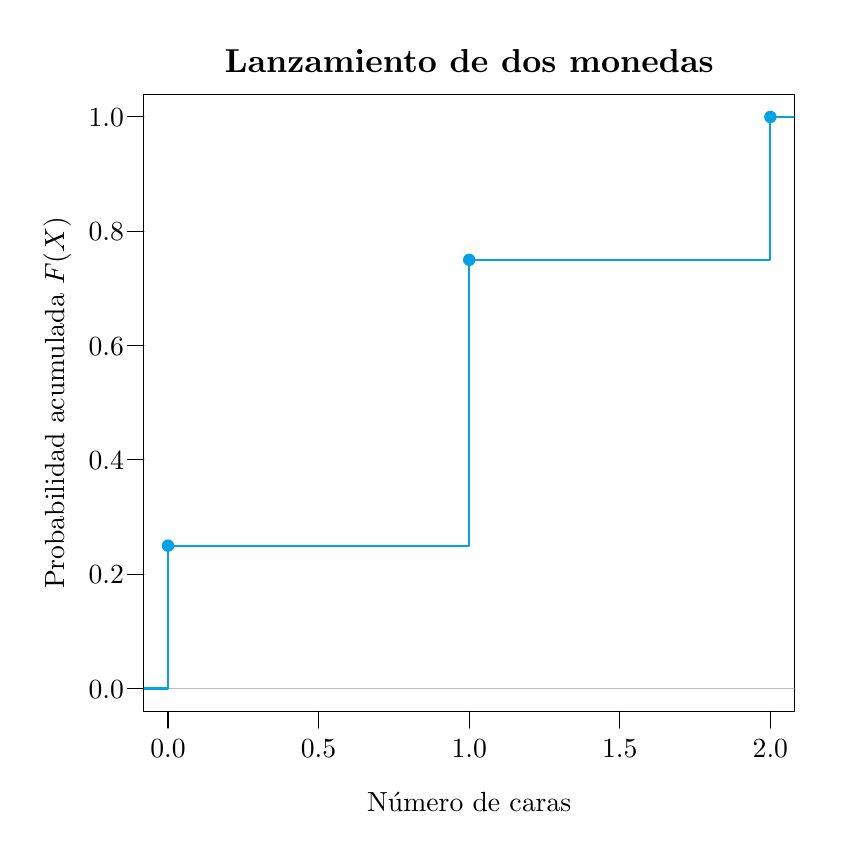
\begin{tikzpicture}[x=1pt,y=1pt]
\definecolor{fillColor}{RGB}{255,255,255}
\path[use as bounding box,fill=fillColor,fill opacity=0.00] (0,0) rectangle (289.08,289.08);
\begin{scope}
\path[clip] ( 42.00, 42.00) rectangle (277.08,265.08);
\definecolor{fillColor}{RGB}{5,161,230}

\path[fill=fillColor] ( 50.71,101.90) circle (  2.25);

\path[fill=fillColor] (159.54,205.18) circle (  2.25);

\path[fill=fillColor] (268.37,256.82) circle (  2.25);
\end{scope}
\begin{scope}
\path[clip] (  0.00,  0.00) rectangle (289.08,289.08);
\definecolor{drawColor}{RGB}{0,0,0}

\path[draw=drawColor,line width= 0.4pt,line join=round,line cap=round] ( 50.71, 42.00) -- (268.37, 42.00);

\path[draw=drawColor,line width= 0.4pt,line join=round,line cap=round] ( 50.71, 42.00) -- ( 50.71, 36.00);

\path[draw=drawColor,line width= 0.4pt,line join=round,line cap=round] (105.12, 42.00) -- (105.12, 36.00);

\path[draw=drawColor,line width= 0.4pt,line join=round,line cap=round] (159.54, 42.00) -- (159.54, 36.00);

\path[draw=drawColor,line width= 0.4pt,line join=round,line cap=round] (213.96, 42.00) -- (213.96, 36.00);

\path[draw=drawColor,line width= 0.4pt,line join=round,line cap=round] (268.37, 42.00) -- (268.37, 36.00);

\node[text=drawColor,anchor=base,inner sep=0pt, outer sep=0pt, scale=  1.00] at ( 50.71, 25.20) {0.0};

\node[text=drawColor,anchor=base,inner sep=0pt, outer sep=0pt, scale=  1.00] at (105.12, 25.20) {0.5};

\node[text=drawColor,anchor=base,inner sep=0pt, outer sep=0pt, scale=  1.00] at (159.54, 25.20) {1.0};

\node[text=drawColor,anchor=base,inner sep=0pt, outer sep=0pt, scale=  1.00] at (213.96, 25.20) {1.5};

\node[text=drawColor,anchor=base,inner sep=0pt, outer sep=0pt, scale=  1.00] at (268.37, 25.20) {2.0};

\path[draw=drawColor,line width= 0.4pt,line join=round,line cap=round] ( 42.00, 50.26) -- ( 42.00,256.82);

\path[draw=drawColor,line width= 0.4pt,line join=round,line cap=round] ( 42.00, 50.26) -- ( 36.00, 50.26);

\path[draw=drawColor,line width= 0.4pt,line join=round,line cap=round] ( 42.00, 91.57) -- ( 36.00, 91.57);

\path[draw=drawColor,line width= 0.4pt,line join=round,line cap=round] ( 42.00,132.88) -- ( 36.00,132.88);

\path[draw=drawColor,line width= 0.4pt,line join=round,line cap=round] ( 42.00,174.20) -- ( 36.00,174.20);

\path[draw=drawColor,line width= 0.4pt,line join=round,line cap=round] ( 42.00,215.51) -- ( 36.00,215.51);

\path[draw=drawColor,line width= 0.4pt,line join=round,line cap=round] ( 42.00,256.82) -- ( 36.00,256.82);

\node[text=drawColor,anchor=base east,inner sep=0pt, outer sep=0pt, scale=  1.00] at ( 34.80, 46.82) {0.0};

\node[text=drawColor,anchor=base east,inner sep=0pt, outer sep=0pt, scale=  1.00] at ( 34.80, 88.13) {0.2};

\node[text=drawColor,anchor=base east,inner sep=0pt, outer sep=0pt, scale=  1.00] at ( 34.80,129.44) {0.4};

\node[text=drawColor,anchor=base east,inner sep=0pt, outer sep=0pt, scale=  1.00] at ( 34.80,170.75) {0.6};

\node[text=drawColor,anchor=base east,inner sep=0pt, outer sep=0pt, scale=  1.00] at ( 34.80,212.06) {0.8};

\node[text=drawColor,anchor=base east,inner sep=0pt, outer sep=0pt, scale=  1.00] at ( 34.80,253.37) {1.0};

\path[draw=drawColor,line width= 0.4pt,line join=round,line cap=round] ( 42.00, 42.00) --
	(277.08, 42.00) --
	(277.08,265.08) --
	( 42.00,265.08) --
	( 42.00, 42.00);
\end{scope}
\begin{scope}
\path[clip] (  0.00,  0.00) rectangle (289.08,289.08);
\definecolor{drawColor}{RGB}{0,0,0}

\node[text=drawColor,anchor=base,inner sep=0pt, outer sep=0pt, scale=  1.20] at (159.54,272.89) {\bfseries Lanzamiento de dos monedas};

\node[text=drawColor,anchor=base,inner sep=0pt, outer sep=0pt, scale=  1.00] at (159.54,  6.00) {Número de caras};

\node[text=drawColor,rotate= 90.00,anchor=base,inner sep=0pt, outer sep=0pt, scale=  1.00] at ( 13.20,153.54) {Probabilidad acumulada $F(X)$};
\end{scope}
\begin{scope}
\path[clip] ( 42.00, 42.00) rectangle (277.08,265.08);
\definecolor{drawColor}{RGB}{190,190,190}

\path[draw=drawColor,line width= 0.4pt,line join=round,line cap=round] ( 42.00, 50.26) -- (277.08, 50.26);
\definecolor{drawColor}{RGB}{5,161,230}

\path[draw=drawColor,line width= 0.8pt,line join=round,line cap=round] (  0.00, 50.26) --
	( 50.71, 50.26) --
	( 50.71,101.90) --
	(159.54,101.90) --
	(159.54,205.18) --
	(268.37,205.18) --
	(268.37,256.82) --
	(289.08,256.82);
\end{scope}
\end{tikzpicture}
}}
	\mode<presentation>{\resizebox{0.45\textwidth}{!}{% Created by tikzDevice version 0.10.1 on 2016-04-19 18:05:39
% !TEX encoding = UTF-8 Unicode
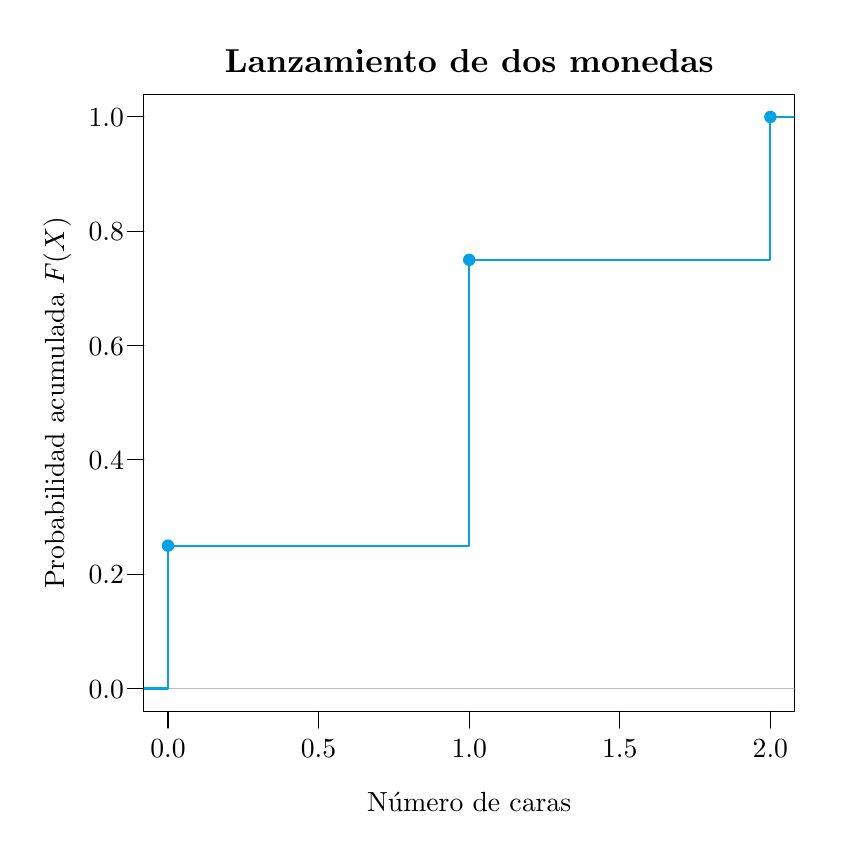
\begin{tikzpicture}[x=1pt,y=1pt]
\definecolor{fillColor}{RGB}{255,255,255}
\path[use as bounding box,fill=fillColor,fill opacity=0.00] (0,0) rectangle (289.08,289.08);
\begin{scope}
\path[clip] ( 42.00, 42.00) rectangle (277.08,265.08);
\definecolor{fillColor}{RGB}{5,161,230}

\path[fill=fillColor] ( 50.71,101.90) circle (  2.25);

\path[fill=fillColor] (159.54,205.18) circle (  2.25);

\path[fill=fillColor] (268.37,256.82) circle (  2.25);
\end{scope}
\begin{scope}
\path[clip] (  0.00,  0.00) rectangle (289.08,289.08);
\definecolor{drawColor}{RGB}{0,0,0}

\path[draw=drawColor,line width= 0.4pt,line join=round,line cap=round] ( 50.71, 42.00) -- (268.37, 42.00);

\path[draw=drawColor,line width= 0.4pt,line join=round,line cap=round] ( 50.71, 42.00) -- ( 50.71, 36.00);

\path[draw=drawColor,line width= 0.4pt,line join=round,line cap=round] (105.12, 42.00) -- (105.12, 36.00);

\path[draw=drawColor,line width= 0.4pt,line join=round,line cap=round] (159.54, 42.00) -- (159.54, 36.00);

\path[draw=drawColor,line width= 0.4pt,line join=round,line cap=round] (213.96, 42.00) -- (213.96, 36.00);

\path[draw=drawColor,line width= 0.4pt,line join=round,line cap=round] (268.37, 42.00) -- (268.37, 36.00);

\node[text=drawColor,anchor=base,inner sep=0pt, outer sep=0pt, scale=  1.00] at ( 50.71, 25.20) {0.0};

\node[text=drawColor,anchor=base,inner sep=0pt, outer sep=0pt, scale=  1.00] at (105.12, 25.20) {0.5};

\node[text=drawColor,anchor=base,inner sep=0pt, outer sep=0pt, scale=  1.00] at (159.54, 25.20) {1.0};

\node[text=drawColor,anchor=base,inner sep=0pt, outer sep=0pt, scale=  1.00] at (213.96, 25.20) {1.5};

\node[text=drawColor,anchor=base,inner sep=0pt, outer sep=0pt, scale=  1.00] at (268.37, 25.20) {2.0};

\path[draw=drawColor,line width= 0.4pt,line join=round,line cap=round] ( 42.00, 50.26) -- ( 42.00,256.82);

\path[draw=drawColor,line width= 0.4pt,line join=round,line cap=round] ( 42.00, 50.26) -- ( 36.00, 50.26);

\path[draw=drawColor,line width= 0.4pt,line join=round,line cap=round] ( 42.00, 91.57) -- ( 36.00, 91.57);

\path[draw=drawColor,line width= 0.4pt,line join=round,line cap=round] ( 42.00,132.88) -- ( 36.00,132.88);

\path[draw=drawColor,line width= 0.4pt,line join=round,line cap=round] ( 42.00,174.20) -- ( 36.00,174.20);

\path[draw=drawColor,line width= 0.4pt,line join=round,line cap=round] ( 42.00,215.51) -- ( 36.00,215.51);

\path[draw=drawColor,line width= 0.4pt,line join=round,line cap=round] ( 42.00,256.82) -- ( 36.00,256.82);

\node[text=drawColor,anchor=base east,inner sep=0pt, outer sep=0pt, scale=  1.00] at ( 34.80, 46.82) {0.0};

\node[text=drawColor,anchor=base east,inner sep=0pt, outer sep=0pt, scale=  1.00] at ( 34.80, 88.13) {0.2};

\node[text=drawColor,anchor=base east,inner sep=0pt, outer sep=0pt, scale=  1.00] at ( 34.80,129.44) {0.4};

\node[text=drawColor,anchor=base east,inner sep=0pt, outer sep=0pt, scale=  1.00] at ( 34.80,170.75) {0.6};

\node[text=drawColor,anchor=base east,inner sep=0pt, outer sep=0pt, scale=  1.00] at ( 34.80,212.06) {0.8};

\node[text=drawColor,anchor=base east,inner sep=0pt, outer sep=0pt, scale=  1.00] at ( 34.80,253.37) {1.0};

\path[draw=drawColor,line width= 0.4pt,line join=round,line cap=round] ( 42.00, 42.00) --
	(277.08, 42.00) --
	(277.08,265.08) --
	( 42.00,265.08) --
	( 42.00, 42.00);
\end{scope}
\begin{scope}
\path[clip] (  0.00,  0.00) rectangle (289.08,289.08);
\definecolor{drawColor}{RGB}{0,0,0}

\node[text=drawColor,anchor=base,inner sep=0pt, outer sep=0pt, scale=  1.20] at (159.54,272.89) {\bfseries Lanzamiento de dos monedas};

\node[text=drawColor,anchor=base,inner sep=0pt, outer sep=0pt, scale=  1.00] at (159.54,  6.00) {Número de caras};

\node[text=drawColor,rotate= 90.00,anchor=base,inner sep=0pt, outer sep=0pt, scale=  1.00] at ( 13.20,153.54) {Probabilidad acumulada $F(X)$};
\end{scope}
\begin{scope}
\path[clip] ( 42.00, 42.00) rectangle (277.08,265.08);
\definecolor{drawColor}{RGB}{190,190,190}

\path[draw=drawColor,line width= 0.4pt,line join=round,line cap=round] ( 42.00, 50.26) -- (277.08, 50.26);
\definecolor{drawColor}{RGB}{5,161,230}

\path[draw=drawColor,line width= 0.8pt,line join=round,line cap=round] (  0.00, 50.26) --
	( 50.71, 50.26) --
	( 50.71,101.90) --
	(159.54,101.90) --
	(159.54,205.18) --
	(268.37,205.18) --
	(268.37,256.82) --
	(289.08,256.82);
\end{scope}
\end{tikzpicture}
}}
	\end{tabular}
\end{center} 

\note{
Tanto la función de probabilidad como la de distribución también suelen representarse gráficamente, de igual modo que representábamos las
frecuencias muestrales.

Como se trata de variables discretas, el diagrama que se utiliza es el diagrama de barras o el diagrama de puntos, donde para cada valor se
levanta una barra con el valor de la función de probabilidad o con el valor de la función de distribución.

En el ejemplo de la variable que mide el número de caras al lanzar dos monedas, se tiene que la gráfica de la función de probabilidad es
la que aparece a la izquierda, mientras que la de la función de distribución es la de la derecha.
}
\end{frame}


%---------------------------------------------------------------------slide----
\begin{frame}
\frametitle{Estadísticos poblacionales}
Al igual que para describir las variables en las muestras se utilizan estadísticos descriptivos muestrales, para describir las características de las variables aleatorias se utilizan también estadísticos poblacionales.

La definición de los estadísticos poblacionales es análoga a la de los muestrales, pero utilizando probabilidades en lugar de frecuencias relativas.

Los más importantes son\footnote{Para distinguirlos de los muestrales se suelen representar con letras griegas}:
\begin{itemize}
\item \structure{Media o esperanza matemática}:
\[
\mu = E(X) = \sum_{i=1}^n x_i f(x_i)
\]
\item \structure{Varianza}:
\[
\sigma^2 = Var(X) = \sum_{i=1}^n x_i^2 f(x_i) -\mu^2
\]
\item \structure{Desviación típica}:
\[
\sigma = +\sqrt{\sigma^2}
\] 
\end{itemize}

\note{
Al igual que para describir las variables medidas en las muestras se utilizan estadísticos descriptivos, para describir determinadas
características de variables aleatorias se utilizan también estadísticos poblacionales.

Los estadísticos poblacionales se representan con letras griegas para distinguirlos de los muestrales, y su definición es análoga a la de
los muestrales, pero utilizando probabilidades en lugar de frecuencias relativas.

Por ejemplo, si definíamos la media muestral como la suma del producto de cada valor por su frecuencia relativa, la media poblacional, que
también se llama esperanza matemática, y se representa por $\mu$, se calcula como la suma del producto de cada valor de la variable por su
probabilidad. 

La varianza poblacional se calcula sumando los productos de los cuadrados de los valores de la variable por su probabilidad y restándole al
total de la suma la media poblacional al cuadrado. 

La desviación típica poblacional, como siempre, es la raíz cuadrada positiva de la varianza poblacional.

Otros estadísticos, se definen de forma similar a como lo hacíamos para muestras. Por ejemplo, la mediana será el valor cuya probabilidad
acumulada sea $0.5$. 
}

\end{frame}


%---------------------------------------------------------------------slide----
\begin{frame}
\frametitle{Estadísticos poblacionales}
\framesubtitle{Ejemplo del lanzamiento de dos monedas}
En el experimento aleatorio del lanzamiento de dos monedas, a partir de la distribución de probabilidad
\[
\begin{array}{|c|ccc|}
\hline
X & 0 & 1 & 2\\ \hline
f(x) & 0.25 & 0.5 & 0.25\\
\hline
F(x) & 0.25 & 0.75 & 1 \\
\hline 
\end{array}
\]
se pueden calcular fácilmente los estadísticos poblacionales
\begin{align*}
\mu &= \sum_{i=1}^n x_i f(x_i) = 0\cdot 0.25 + 1\cdot 0.5 + 2\cdot 0.25 = 1 \mbox{ cara},\\
\sigma^2 &= \sum_{i=1}^n x_i^2 f(x_i) -\mu^2 = (0^0\cdot 0.25 + 1^2\cdot 0.5 + 2^2\cdot 0.25) - 1^2 = 0.5 \mbox{ caras}^2,\\
\sigma &= +\sqrt{0.5} = 0.71 \mbox{ caras}.
\end{align*} 

\note{
Veamos cómo calcular los principales estadísticos de la variable que medía el número de caras en el lanzamiento de dos monedas. 
}
\end{frame}


%---------------------------------------------------------------------slide----
\begin{frame}
\frametitle{Modelos de distribución de probabilidad}
De acuerdo al tipo de experimento en el que se mide la variable aleatoria, existen diferentes modelos de distribución de probabilidad. 
Los más importantes son
\begin{itemize}
\item Distribución Uniforme.
\item Distribución Binomial.
\item Distribución de Poisson.
\end{itemize}

\note{
En teoría, para obtener la distribución de probabilidad de una variable aleatoria en una población es necesario conocer el valor de la
variable en todos los individuos de la población, lo cual muchas es imposible la mayoría de las veces.

Sin embargo, dependiendo de la naturaleza del experimento, a veces es posible obtener la distribución de probabilidad de una variable
aleatoria sin medirla en toda la población.

Dependiendo del tipo de experimento, existen diferentes modelos de distribución de probabilidad discretos. Los más habituales son:
\begin{itemize}
\item Distribución Uniforme.
\item Distribución Binomial.
\item Distribución de Poisson.
\end{itemize}

A continuación los veremos uno por uno.
}
\end{frame}


\subsection{Distribución Uniforme discreta}

% ---------------------------------------------------------------------slide----
\begin{frame}
\frametitle{Distribución Uniforme $U(a,b)$}
Cuando por la simetría del experimento, todos los valores $a=x_1,\ldots,x_k=b$ de una variable discreta $X$ son igualmente probables, se dice que la variable sigue un \emph{modelo de distribución uniforme}.

\begin{definicion}[Distribución uniforme $U(a,b)$]
Se dice que una variable aleatoria $X$ sigue un \emph{modelo de distribución uniforme} de parámetros $a,b$, y se nota $X\sim U(a,b)$, si su rango es $Ran(X) = \{a, a+1, \ldots,b\}$, y su función de probabilidad vale
\[
  f(x)=\frac{1}{b-a+1}.
\]
\end{definicion}

Obsérvese que $a$ y $b$ son el mínimo y el máximo del rango respectivamente.

Su media y varianza valen
\[
  \mu = \sum_{i=0}^{b-a}\frac{a+i}{b-a+1}=\frac{a+b}{2} \qquad \sigma^2 =\sum_{i=0}^{b-a}\frac{(a+i-\mu)^2}{b-a+1}=
  \frac{(b-a+1)^2-1}{12}
\]

\note{
Cuando por la simetría del experimento, todos los valores $a=x_1,\ldots,x_k=b$ de una variable discreta $X$ son igualmente probables, se
dice que la variable sigue un \emph{modelo de distribución uniforme}.

\begin{definicion}[Distribución uniforme $U(a,b)$]
Se dice que una variable aleatoria $X$ sigue un \emph{modelo de distribución uniforme} de parámetros $a,b$, y se nota,
$X\sim U(a,b)$, si puede tomar $k$ valores distintos desde $a$ hasta $b$, es decir, su recorrido es $Re(X) = \{a=x_1,\ldots,x_k=b\}$, y su
función de probabilidad de cada uno de estos valores es la misma, es decir,  \[f(x_i)=\frac{1}{k}.\]
\end{definicion}

Su media, valdrá, por tanto, 
\[
\mu = \sum_{i=1}^{k}x_i\frac{1}{k}.
\]
y su varianza
\[
\sigma^2 =\sum_{i=1}^k (x_i-\mu)^2\frac{1}{k}.
\]
}
\end{frame}


%---------------------------------------------------------------------slide----
\begin{frame}
\frametitle{Distribución Uniforme $U(a,b)$}
\framesubtitle{Ejemplo del lanzamiento de un dado}
La variable que mide el número obtenido al lanzar un dado sigue un modelo de distribución uniforme $U(1,6)$.
\begin{center}
  \tikzsetnextfilename{variables_aleatorias_discretas/funcion_probabilidad_uniforme_discreta}
  \mode<article>{\resizebox{0.5\textwidth}{!}{% Created by tikzDevice version 0.10.1 on 2016-04-19 18:05:41
% !TEX encoding = UTF-8 Unicode
\begin{tikzpicture}[x=1pt,y=1pt]
\definecolor{fillColor}{RGB}{255,255,255}
\path[use as bounding box,fill=fillColor,fill opacity=0.00] (0,0) rectangle (289.08,289.08);
\begin{scope}
\path[clip] ( 42.00, 42.00) rectangle (277.08,265.08);
\definecolor{fillColor}{RGB}{5,161,230}

\path[fill=fillColor] ( 50.71,222.39) circle (  2.25);

\path[fill=fillColor] ( 94.24,222.39) circle (  2.25);

\path[fill=fillColor] (137.77,222.39) circle (  2.25);

\path[fill=fillColor] (181.31,222.39) circle (  2.25);

\path[fill=fillColor] (224.84,222.39) circle (  2.25);

\path[fill=fillColor] (268.37,222.39) circle (  2.25);
\end{scope}
\begin{scope}
\path[clip] (  0.00,  0.00) rectangle (289.08,289.08);
\definecolor{drawColor}{RGB}{0,0,0}

\path[draw=drawColor,line width= 0.4pt,line join=round,line cap=round] ( 50.71, 42.00) -- (268.37, 42.00);

\path[draw=drawColor,line width= 0.4pt,line join=round,line cap=round] ( 50.71, 42.00) -- ( 50.71, 36.00);

\path[draw=drawColor,line width= 0.4pt,line join=round,line cap=round] ( 94.24, 42.00) -- ( 94.24, 36.00);

\path[draw=drawColor,line width= 0.4pt,line join=round,line cap=round] (137.77, 42.00) -- (137.77, 36.00);

\path[draw=drawColor,line width= 0.4pt,line join=round,line cap=round] (181.31, 42.00) -- (181.31, 36.00);

\path[draw=drawColor,line width= 0.4pt,line join=round,line cap=round] (224.84, 42.00) -- (224.84, 36.00);

\path[draw=drawColor,line width= 0.4pt,line join=round,line cap=round] (268.37, 42.00) -- (268.37, 36.00);

\node[text=drawColor,anchor=base,inner sep=0pt, outer sep=0pt, scale=  1.00] at ( 50.71, 25.20) {1};

\node[text=drawColor,anchor=base,inner sep=0pt, outer sep=0pt, scale=  1.00] at ( 94.24, 25.20) {2};

\node[text=drawColor,anchor=base,inner sep=0pt, outer sep=0pt, scale=  1.00] at (137.77, 25.20) {3};

\node[text=drawColor,anchor=base,inner sep=0pt, outer sep=0pt, scale=  1.00] at (181.31, 25.20) {4};

\node[text=drawColor,anchor=base,inner sep=0pt, outer sep=0pt, scale=  1.00] at (224.84, 25.20) {5};

\node[text=drawColor,anchor=base,inner sep=0pt, outer sep=0pt, scale=  1.00] at (268.37, 25.20) {6};

\path[draw=drawColor,line width= 0.4pt,line join=round,line cap=round] ( 42.00, 50.26) -- ( 42.00,256.82);

\path[draw=drawColor,line width= 0.4pt,line join=round,line cap=round] ( 42.00, 50.26) -- ( 36.00, 50.26);

\path[draw=drawColor,line width= 0.4pt,line join=round,line cap=round] ( 42.00,101.90) -- ( 36.00,101.90);

\path[draw=drawColor,line width= 0.4pt,line join=round,line cap=round] ( 42.00,153.54) -- ( 36.00,153.54);

\path[draw=drawColor,line width= 0.4pt,line join=round,line cap=round] ( 42.00,205.18) -- ( 36.00,205.18);

\path[draw=drawColor,line width= 0.4pt,line join=round,line cap=round] ( 42.00,256.82) -- ( 36.00,256.82);

\node[text=drawColor,anchor=base east,inner sep=0pt, outer sep=0pt, scale=  1.00] at ( 34.80, 46.82) {0.00};

\node[text=drawColor,anchor=base east,inner sep=0pt, outer sep=0pt, scale=  1.00] at ( 34.80, 98.46) {0.05};

\node[text=drawColor,anchor=base east,inner sep=0pt, outer sep=0pt, scale=  1.00] at ( 34.80,150.10) {0.10};

\node[text=drawColor,anchor=base east,inner sep=0pt, outer sep=0pt, scale=  1.00] at ( 34.80,201.73) {0.15};

\node[text=drawColor,anchor=base east,inner sep=0pt, outer sep=0pt, scale=  1.00] at ( 34.80,253.37) {0.20};

\path[draw=drawColor,line width= 0.4pt,line join=round,line cap=round] ( 42.00, 42.00) --
	(277.08, 42.00) --
	(277.08,265.08) --
	( 42.00,265.08) --
	( 42.00, 42.00);
\end{scope}
\begin{scope}
\path[clip] (  0.00,  0.00) rectangle (289.08,289.08);
\definecolor{drawColor}{RGB}{0,0,0}

\node[text=drawColor,anchor=base,inner sep=0pt, outer sep=0pt, scale=  1.20] at (159.54,272.89) {\bfseries Distribución Uniforme discreta U(1,6)};

\node[text=drawColor,anchor=base,inner sep=0pt, outer sep=0pt, scale=  1.00] at (159.54,  6.00) {X};

\node[text=drawColor,rotate= 90.00,anchor=base,inner sep=0pt, outer sep=0pt, scale=  1.00] at ( 13.20,153.54) {Probabilidad $f(x)$};
\end{scope}
\begin{scope}
\path[clip] ( 42.00, 42.00) rectangle (277.08,265.08);
\definecolor{drawColor}{RGB}{190,190,190}

\path[draw=drawColor,line width= 0.4pt,line join=round,line cap=round] ( 42.00, 50.26) -- (277.08, 50.26);
\end{scope}
\end{tikzpicture}
}}
  \mode<presentation>{\resizebox{0.6\textwidth}{!}{% Created by tikzDevice version 0.10.1 on 2016-04-19 18:05:41
% !TEX encoding = UTF-8 Unicode
\begin{tikzpicture}[x=1pt,y=1pt]
\definecolor{fillColor}{RGB}{255,255,255}
\path[use as bounding box,fill=fillColor,fill opacity=0.00] (0,0) rectangle (289.08,289.08);
\begin{scope}
\path[clip] ( 42.00, 42.00) rectangle (277.08,265.08);
\definecolor{fillColor}{RGB}{5,161,230}

\path[fill=fillColor] ( 50.71,222.39) circle (  2.25);

\path[fill=fillColor] ( 94.24,222.39) circle (  2.25);

\path[fill=fillColor] (137.77,222.39) circle (  2.25);

\path[fill=fillColor] (181.31,222.39) circle (  2.25);

\path[fill=fillColor] (224.84,222.39) circle (  2.25);

\path[fill=fillColor] (268.37,222.39) circle (  2.25);
\end{scope}
\begin{scope}
\path[clip] (  0.00,  0.00) rectangle (289.08,289.08);
\definecolor{drawColor}{RGB}{0,0,0}

\path[draw=drawColor,line width= 0.4pt,line join=round,line cap=round] ( 50.71, 42.00) -- (268.37, 42.00);

\path[draw=drawColor,line width= 0.4pt,line join=round,line cap=round] ( 50.71, 42.00) -- ( 50.71, 36.00);

\path[draw=drawColor,line width= 0.4pt,line join=round,line cap=round] ( 94.24, 42.00) -- ( 94.24, 36.00);

\path[draw=drawColor,line width= 0.4pt,line join=round,line cap=round] (137.77, 42.00) -- (137.77, 36.00);

\path[draw=drawColor,line width= 0.4pt,line join=round,line cap=round] (181.31, 42.00) -- (181.31, 36.00);

\path[draw=drawColor,line width= 0.4pt,line join=round,line cap=round] (224.84, 42.00) -- (224.84, 36.00);

\path[draw=drawColor,line width= 0.4pt,line join=round,line cap=round] (268.37, 42.00) -- (268.37, 36.00);

\node[text=drawColor,anchor=base,inner sep=0pt, outer sep=0pt, scale=  1.00] at ( 50.71, 25.20) {1};

\node[text=drawColor,anchor=base,inner sep=0pt, outer sep=0pt, scale=  1.00] at ( 94.24, 25.20) {2};

\node[text=drawColor,anchor=base,inner sep=0pt, outer sep=0pt, scale=  1.00] at (137.77, 25.20) {3};

\node[text=drawColor,anchor=base,inner sep=0pt, outer sep=0pt, scale=  1.00] at (181.31, 25.20) {4};

\node[text=drawColor,anchor=base,inner sep=0pt, outer sep=0pt, scale=  1.00] at (224.84, 25.20) {5};

\node[text=drawColor,anchor=base,inner sep=0pt, outer sep=0pt, scale=  1.00] at (268.37, 25.20) {6};

\path[draw=drawColor,line width= 0.4pt,line join=round,line cap=round] ( 42.00, 50.26) -- ( 42.00,256.82);

\path[draw=drawColor,line width= 0.4pt,line join=round,line cap=round] ( 42.00, 50.26) -- ( 36.00, 50.26);

\path[draw=drawColor,line width= 0.4pt,line join=round,line cap=round] ( 42.00,101.90) -- ( 36.00,101.90);

\path[draw=drawColor,line width= 0.4pt,line join=round,line cap=round] ( 42.00,153.54) -- ( 36.00,153.54);

\path[draw=drawColor,line width= 0.4pt,line join=round,line cap=round] ( 42.00,205.18) -- ( 36.00,205.18);

\path[draw=drawColor,line width= 0.4pt,line join=round,line cap=round] ( 42.00,256.82) -- ( 36.00,256.82);

\node[text=drawColor,anchor=base east,inner sep=0pt, outer sep=0pt, scale=  1.00] at ( 34.80, 46.82) {0.00};

\node[text=drawColor,anchor=base east,inner sep=0pt, outer sep=0pt, scale=  1.00] at ( 34.80, 98.46) {0.05};

\node[text=drawColor,anchor=base east,inner sep=0pt, outer sep=0pt, scale=  1.00] at ( 34.80,150.10) {0.10};

\node[text=drawColor,anchor=base east,inner sep=0pt, outer sep=0pt, scale=  1.00] at ( 34.80,201.73) {0.15};

\node[text=drawColor,anchor=base east,inner sep=0pt, outer sep=0pt, scale=  1.00] at ( 34.80,253.37) {0.20};

\path[draw=drawColor,line width= 0.4pt,line join=round,line cap=round] ( 42.00, 42.00) --
	(277.08, 42.00) --
	(277.08,265.08) --
	( 42.00,265.08) --
	( 42.00, 42.00);
\end{scope}
\begin{scope}
\path[clip] (  0.00,  0.00) rectangle (289.08,289.08);
\definecolor{drawColor}{RGB}{0,0,0}

\node[text=drawColor,anchor=base,inner sep=0pt, outer sep=0pt, scale=  1.20] at (159.54,272.89) {\bfseries Distribución Uniforme discreta U(1,6)};

\node[text=drawColor,anchor=base,inner sep=0pt, outer sep=0pt, scale=  1.00] at (159.54,  6.00) {X};

\node[text=drawColor,rotate= 90.00,anchor=base,inner sep=0pt, outer sep=0pt, scale=  1.00] at ( 13.20,153.54) {Probabilidad $f(x)$};
\end{scope}
\begin{scope}
\path[clip] ( 42.00, 42.00) rectangle (277.08,265.08);
\definecolor{drawColor}{RGB}{190,190,190}

\path[draw=drawColor,line width= 0.4pt,line join=round,line cap=round] ( 42.00, 50.26) -- (277.08, 50.26);
\end{scope}
\end{tikzpicture}
}}
\end{center}

\note{
Un ejemplo sencillo de variable con distribución uniforme es la que mide el resultado del lanzamiento de un dado. Como puede tomar 6 valores
distintos del 1 al 6, su función de probabilidad es constante vale $1/6$ para cualquier valor, tal y como se aprecia en la gráfica.

El modelo de distribución uniforme es el más sencillo, pero resulta poco útil en la práctica ya que la equiprobabilidad no suele cumplirse
fuera de los juegos de azar.
}
\end{frame}


\subsection{Distribución Binomial}

%---------------------------------------------------------------------slide----
\begin{frame}
\frametitle{Distribución Binomial}
La distribución binomial corresponde a una variable aleatoria medida en un experimento aleatorio con las siguientes características:
\begin{itemize}
\item El experimento consiste en una secuencia de $n$ repeticiones de un mismo ensayo aleatorio.
\item Los ensayos se realizan bajo idénticas condiciones, y cada uno de ellos tiene únicamente dos posibles resultados conocidos como \emph{Éxito} o \emph{Fracaso}.
\item Los ensayos son independientes.
\item La probabilidad de éxito es idéntica para todos los ensayos y vale $P(\mbox{Éxisto})=p$.
\end{itemize}

En estas condiciones, la variable aleatoria $X$ que mide le número de éxitos obtenidos en los $n$ ensayos sigue un \emph{modelo de distribución binomial} de parámetros $n$ y $p$.

\note{
Mucho más habitual es el modelo binomial, que suele darse en experimentos aleatorios con las siguientes características:
\begin{itemize}
\item El experimento consiste en una secuencia de $n$ repeticiones de un mismo ensayo aleatorio. Por ejemplo, tirar 10 veces una moneda. 
\item Los ensayos se realizan bajo idénticas condiciones, y cada uno de ellos tiene únicamente dos posibles resultados,
que habitualmente se denotan por éxito ($A$) o fracaso ($\overline A$). Por ejemplo, medir en cada lanzamiento si sale cara (éxito) o si
sale cruz (fracaso).
\item Los ensayos son independientes, por lo que el resultado de cualquier ensayo en particular no influye sobre el resultado de cualquier
otro. Por ejemplo, el resultado de cada lanzamiento de la moneda no depende de los otros.
\item La probabilidad de éxito es idéntica para todos los ensayos y vale $P(A)=p$. Por ejemplo, la probabilidad de sacar cara es $0.5$ en
todos los lanzamientos. 
\end{itemize}
En estas condiciones, la variable aleatoria $X$ que mide le número de éxitos obtenidos en los $n$ ensayos sigue un
\emph{modelo de distribución binomial} de parámetros $n$ y $p$, donde $n$ era el número de repeticiones del ensayo y $p$ es la probabilidad
de lo que llamemos éxito. Así, la variable que mide el número de caras obtenidas en 10 lanzamientos de una moneda es sigue un modelo de
distribución binomial de parámetros $n=10$ y $p=0.5$.

}
\end{frame}


%---------------------------------------------------------------------slide----
\begin{frame}
\frametitle{Distribución Binomial $B(n,p)$}
\begin{definicion}[Distribución Binomial $(B(n,p)$]
Se dice que una variable aleatoria $X$ sigue un \emph{modelo de distribución binomial} de parámetros $n$ y $p$, y se nota $X\sim B(n,p)$, si su recorrido es $Ran(X) =
\{0,1,\ldots,n\}$ y su función de probabilidad vale
\[
f(x) = \binom{n}{x}p^x(1-p)^{n-x} = \frac{n!}{x!(n-x)!}p^x(1-p)^{n-x}.
\]
\end{definicion}

Obsérvese que $n$ es conocido como el número de repeticiones de la prueba o ensayo y $p$ como la probabilidad de Éxito en cada repetición.

Su media y varianza valen
\[
\mu = n\cdot p \qquad \sigma^2 = n\cdot p\cdot (1-p).
\]

\note{
Una variable con distribución binomial cumple que su recorrido va de $0$ a $n$ y su función de probablidad viene dada por la fórmula
\[
f(x) = \binom{n}{x}p^x(1-p)^{n-x}.
\]
donde el número combinatorio $\binom{n}{x}$ se define como $\frac{n!}{x!(n-x)!}$ y $n!$ es el producto de todos los números consecutivos
desde $1$ hasta $n$.

Se cumple además que su media es 
\[
\mu = n\cdot p.
\]
y su varianza
\[
\sigma^2 = n\cdot p\cdot (1-p).
\]
}
\end{frame}


%---------------------------------------------------------------------slide----
\begin{frame}
\frametitle{Distribución Binomial $B(n,p)$}
\framesubtitle{Ejemplo de 10 lanzamientos de una moneda}
La variable que mide el número de caras obtenidos al lanzar 10 veces una moneda sigue un modelo de distribución binomial $B(10,\,0.5)$.
\begin{center}
  \tikzsetnextfilename{variables_aleatorias_discretas/funcion_probabilidad_binomial}
  \mode<article>{\resizebox{0.5\textwidth}{!}{% Created by tikzDevice version 0.10.1 on 2016-04-19 18:05:47
% !TEX encoding = UTF-8 Unicode
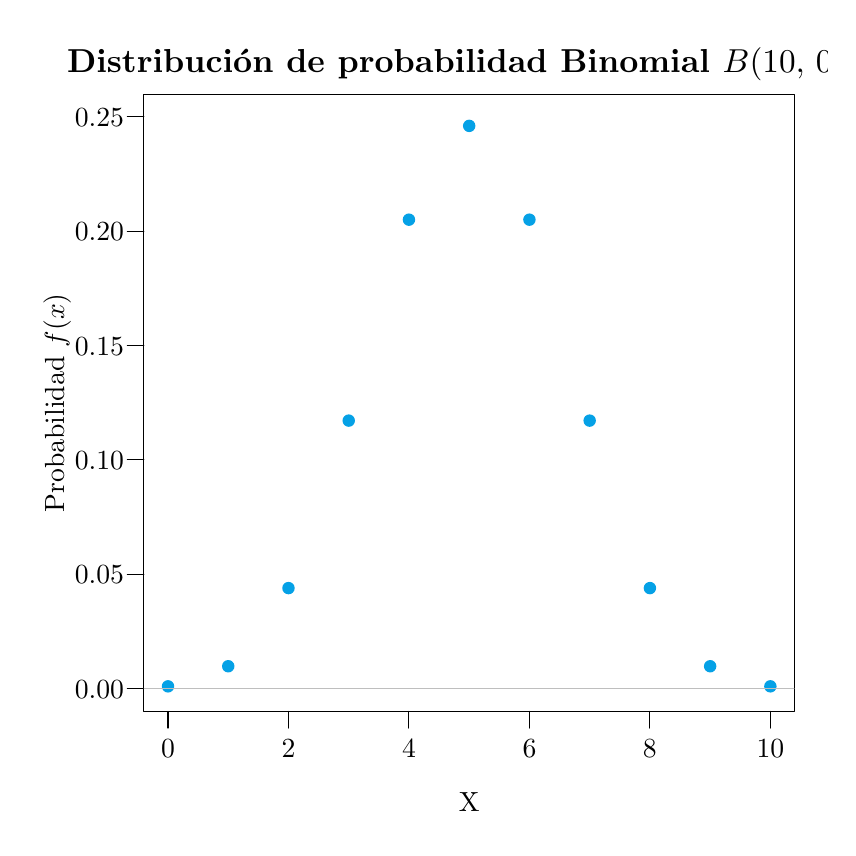
\begin{tikzpicture}[x=1pt,y=1pt]
\definecolor{fillColor}{RGB}{255,255,255}
\path[use as bounding box,fill=fillColor,fill opacity=0.00] (0,0) rectangle (289.08,289.08);
\begin{scope}
\path[clip] ( 42.00, 42.00) rectangle (277.08,265.08);
\definecolor{fillColor}{RGB}{5,161,230}

\path[fill=fillColor] ( 50.71, 51.07) circle (  2.25);

\path[fill=fillColor] ( 72.47, 58.33) circle (  2.25);

\path[fill=fillColor] ( 94.24, 86.57) circle (  2.25);

\path[fill=fillColor] (116.01,147.09) circle (  2.25);

\path[fill=fillColor] (137.77,219.70) circle (  2.25);

\path[fill=fillColor] (159.54,253.59) circle (  2.25);

\path[fill=fillColor] (181.31,219.70) circle (  2.25);

\path[fill=fillColor] (203.07,147.09) circle (  2.25);

\path[fill=fillColor] (224.84, 86.57) circle (  2.25);

\path[fill=fillColor] (246.61, 58.33) circle (  2.25);

\path[fill=fillColor] (268.37, 51.07) circle (  2.25);
\end{scope}
\begin{scope}
\path[clip] (  0.00,  0.00) rectangle (289.08,289.08);
\definecolor{drawColor}{RGB}{0,0,0}

\path[draw=drawColor,line width= 0.4pt,line join=round,line cap=round] ( 50.71, 42.00) -- (268.37, 42.00);

\path[draw=drawColor,line width= 0.4pt,line join=round,line cap=round] ( 50.71, 42.00) -- ( 50.71, 36.00);

\path[draw=drawColor,line width= 0.4pt,line join=round,line cap=round] ( 94.24, 42.00) -- ( 94.24, 36.00);

\path[draw=drawColor,line width= 0.4pt,line join=round,line cap=round] (137.77, 42.00) -- (137.77, 36.00);

\path[draw=drawColor,line width= 0.4pt,line join=round,line cap=round] (181.31, 42.00) -- (181.31, 36.00);

\path[draw=drawColor,line width= 0.4pt,line join=round,line cap=round] (224.84, 42.00) -- (224.84, 36.00);

\path[draw=drawColor,line width= 0.4pt,line join=round,line cap=round] (268.37, 42.00) -- (268.37, 36.00);

\node[text=drawColor,anchor=base,inner sep=0pt, outer sep=0pt, scale=  1.00] at ( 50.71, 25.20) {0};

\node[text=drawColor,anchor=base,inner sep=0pt, outer sep=0pt, scale=  1.00] at ( 94.24, 25.20) {2};

\node[text=drawColor,anchor=base,inner sep=0pt, outer sep=0pt, scale=  1.00] at (137.77, 25.20) {4};

\node[text=drawColor,anchor=base,inner sep=0pt, outer sep=0pt, scale=  1.00] at (181.31, 25.20) {6};

\node[text=drawColor,anchor=base,inner sep=0pt, outer sep=0pt, scale=  1.00] at (224.84, 25.20) {8};

\node[text=drawColor,anchor=base,inner sep=0pt, outer sep=0pt, scale=  1.00] at (268.37, 25.20) {10};

\path[draw=drawColor,line width= 0.4pt,line join=round,line cap=round] ( 42.00, 50.26) -- ( 42.00,256.82);

\path[draw=drawColor,line width= 0.4pt,line join=round,line cap=round] ( 42.00, 50.26) -- ( 36.00, 50.26);

\path[draw=drawColor,line width= 0.4pt,line join=round,line cap=round] ( 42.00, 91.57) -- ( 36.00, 91.57);

\path[draw=drawColor,line width= 0.4pt,line join=round,line cap=round] ( 42.00,132.88) -- ( 36.00,132.88);

\path[draw=drawColor,line width= 0.4pt,line join=round,line cap=round] ( 42.00,174.20) -- ( 36.00,174.20);

\path[draw=drawColor,line width= 0.4pt,line join=round,line cap=round] ( 42.00,215.51) -- ( 36.00,215.51);

\path[draw=drawColor,line width= 0.4pt,line join=round,line cap=round] ( 42.00,256.82) -- ( 36.00,256.82);

\node[text=drawColor,anchor=base east,inner sep=0pt, outer sep=0pt, scale=  1.00] at ( 34.80, 46.82) {0.00};

\node[text=drawColor,anchor=base east,inner sep=0pt, outer sep=0pt, scale=  1.00] at ( 34.80, 88.13) {0.05};

\node[text=drawColor,anchor=base east,inner sep=0pt, outer sep=0pt, scale=  1.00] at ( 34.80,129.44) {0.10};

\node[text=drawColor,anchor=base east,inner sep=0pt, outer sep=0pt, scale=  1.00] at ( 34.80,170.75) {0.15};

\node[text=drawColor,anchor=base east,inner sep=0pt, outer sep=0pt, scale=  1.00] at ( 34.80,212.06) {0.20};

\node[text=drawColor,anchor=base east,inner sep=0pt, outer sep=0pt, scale=  1.00] at ( 34.80,253.37) {0.25};

\path[draw=drawColor,line width= 0.4pt,line join=round,line cap=round] ( 42.00, 42.00) --
	(277.08, 42.00) --
	(277.08,265.08) --
	( 42.00,265.08) --
	( 42.00, 42.00);
\end{scope}
\begin{scope}
\path[clip] (  0.00,  0.00) rectangle (289.08,289.08);
\definecolor{drawColor}{RGB}{0,0,0}

\node[text=drawColor,anchor=base,inner sep=0pt, outer sep=0pt, scale=  1.20] at (159.54,272.89) {\bfseries Distribución de probabilidad Binomial $B(10,\,0.5)$};

\node[text=drawColor,anchor=base,inner sep=0pt, outer sep=0pt, scale=  1.00] at (159.54,  6.00) {X};

\node[text=drawColor,rotate= 90.00,anchor=base,inner sep=0pt, outer sep=0pt, scale=  1.00] at ( 13.20,153.54) {Probabilidad $f(x)$};
\end{scope}
\begin{scope}
\path[clip] ( 42.00, 42.00) rectangle (277.08,265.08);
\definecolor{drawColor}{RGB}{190,190,190}

\path[draw=drawColor,line width= 0.4pt,line join=round,line cap=round] ( 42.00, 50.26) -- (277.08, 50.26);
\end{scope}
\end{tikzpicture}
}}
  \mode<presentation>{\resizebox{0.6\textwidth}{!}{% Created by tikzDevice version 0.10.1 on 2016-04-19 18:05:47
% !TEX encoding = UTF-8 Unicode
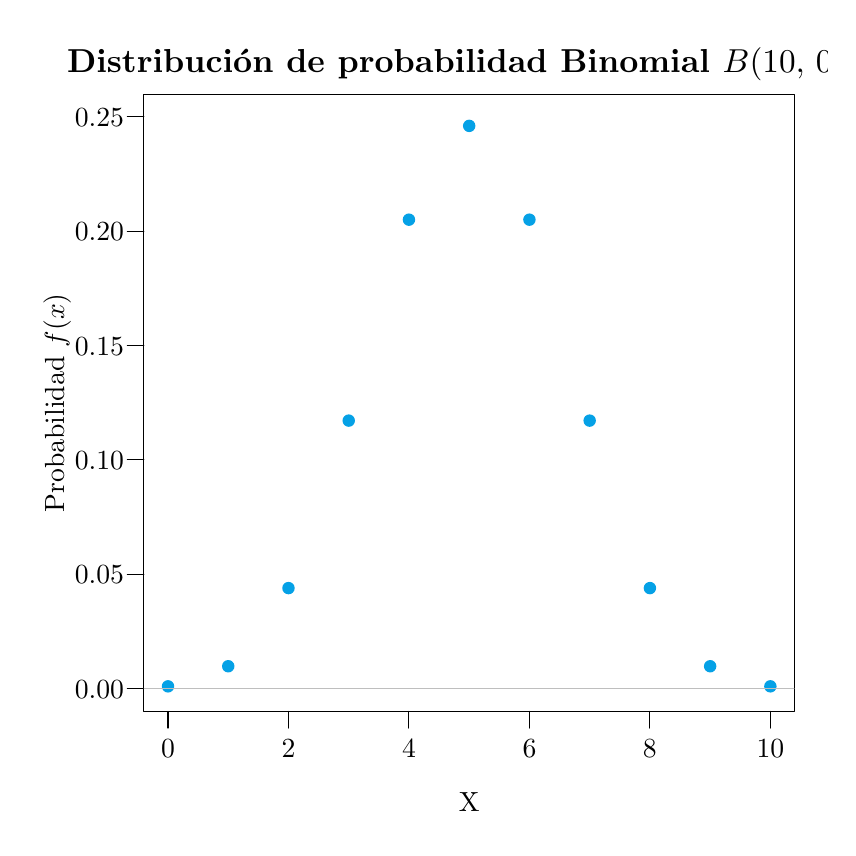
\begin{tikzpicture}[x=1pt,y=1pt]
\definecolor{fillColor}{RGB}{255,255,255}
\path[use as bounding box,fill=fillColor,fill opacity=0.00] (0,0) rectangle (289.08,289.08);
\begin{scope}
\path[clip] ( 42.00, 42.00) rectangle (277.08,265.08);
\definecolor{fillColor}{RGB}{5,161,230}

\path[fill=fillColor] ( 50.71, 51.07) circle (  2.25);

\path[fill=fillColor] ( 72.47, 58.33) circle (  2.25);

\path[fill=fillColor] ( 94.24, 86.57) circle (  2.25);

\path[fill=fillColor] (116.01,147.09) circle (  2.25);

\path[fill=fillColor] (137.77,219.70) circle (  2.25);

\path[fill=fillColor] (159.54,253.59) circle (  2.25);

\path[fill=fillColor] (181.31,219.70) circle (  2.25);

\path[fill=fillColor] (203.07,147.09) circle (  2.25);

\path[fill=fillColor] (224.84, 86.57) circle (  2.25);

\path[fill=fillColor] (246.61, 58.33) circle (  2.25);

\path[fill=fillColor] (268.37, 51.07) circle (  2.25);
\end{scope}
\begin{scope}
\path[clip] (  0.00,  0.00) rectangle (289.08,289.08);
\definecolor{drawColor}{RGB}{0,0,0}

\path[draw=drawColor,line width= 0.4pt,line join=round,line cap=round] ( 50.71, 42.00) -- (268.37, 42.00);

\path[draw=drawColor,line width= 0.4pt,line join=round,line cap=round] ( 50.71, 42.00) -- ( 50.71, 36.00);

\path[draw=drawColor,line width= 0.4pt,line join=round,line cap=round] ( 94.24, 42.00) -- ( 94.24, 36.00);

\path[draw=drawColor,line width= 0.4pt,line join=round,line cap=round] (137.77, 42.00) -- (137.77, 36.00);

\path[draw=drawColor,line width= 0.4pt,line join=round,line cap=round] (181.31, 42.00) -- (181.31, 36.00);

\path[draw=drawColor,line width= 0.4pt,line join=round,line cap=round] (224.84, 42.00) -- (224.84, 36.00);

\path[draw=drawColor,line width= 0.4pt,line join=round,line cap=round] (268.37, 42.00) -- (268.37, 36.00);

\node[text=drawColor,anchor=base,inner sep=0pt, outer sep=0pt, scale=  1.00] at ( 50.71, 25.20) {0};

\node[text=drawColor,anchor=base,inner sep=0pt, outer sep=0pt, scale=  1.00] at ( 94.24, 25.20) {2};

\node[text=drawColor,anchor=base,inner sep=0pt, outer sep=0pt, scale=  1.00] at (137.77, 25.20) {4};

\node[text=drawColor,anchor=base,inner sep=0pt, outer sep=0pt, scale=  1.00] at (181.31, 25.20) {6};

\node[text=drawColor,anchor=base,inner sep=0pt, outer sep=0pt, scale=  1.00] at (224.84, 25.20) {8};

\node[text=drawColor,anchor=base,inner sep=0pt, outer sep=0pt, scale=  1.00] at (268.37, 25.20) {10};

\path[draw=drawColor,line width= 0.4pt,line join=round,line cap=round] ( 42.00, 50.26) -- ( 42.00,256.82);

\path[draw=drawColor,line width= 0.4pt,line join=round,line cap=round] ( 42.00, 50.26) -- ( 36.00, 50.26);

\path[draw=drawColor,line width= 0.4pt,line join=round,line cap=round] ( 42.00, 91.57) -- ( 36.00, 91.57);

\path[draw=drawColor,line width= 0.4pt,line join=round,line cap=round] ( 42.00,132.88) -- ( 36.00,132.88);

\path[draw=drawColor,line width= 0.4pt,line join=round,line cap=round] ( 42.00,174.20) -- ( 36.00,174.20);

\path[draw=drawColor,line width= 0.4pt,line join=round,line cap=round] ( 42.00,215.51) -- ( 36.00,215.51);

\path[draw=drawColor,line width= 0.4pt,line join=round,line cap=round] ( 42.00,256.82) -- ( 36.00,256.82);

\node[text=drawColor,anchor=base east,inner sep=0pt, outer sep=0pt, scale=  1.00] at ( 34.80, 46.82) {0.00};

\node[text=drawColor,anchor=base east,inner sep=0pt, outer sep=0pt, scale=  1.00] at ( 34.80, 88.13) {0.05};

\node[text=drawColor,anchor=base east,inner sep=0pt, outer sep=0pt, scale=  1.00] at ( 34.80,129.44) {0.10};

\node[text=drawColor,anchor=base east,inner sep=0pt, outer sep=0pt, scale=  1.00] at ( 34.80,170.75) {0.15};

\node[text=drawColor,anchor=base east,inner sep=0pt, outer sep=0pt, scale=  1.00] at ( 34.80,212.06) {0.20};

\node[text=drawColor,anchor=base east,inner sep=0pt, outer sep=0pt, scale=  1.00] at ( 34.80,253.37) {0.25};

\path[draw=drawColor,line width= 0.4pt,line join=round,line cap=round] ( 42.00, 42.00) --
	(277.08, 42.00) --
	(277.08,265.08) --
	( 42.00,265.08) --
	( 42.00, 42.00);
\end{scope}
\begin{scope}
\path[clip] (  0.00,  0.00) rectangle (289.08,289.08);
\definecolor{drawColor}{RGB}{0,0,0}

\node[text=drawColor,anchor=base,inner sep=0pt, outer sep=0pt, scale=  1.20] at (159.54,272.89) {\bfseries Distribución de probabilidad Binomial $B(10,\,0.5)$};

\node[text=drawColor,anchor=base,inner sep=0pt, outer sep=0pt, scale=  1.00] at (159.54,  6.00) {X};

\node[text=drawColor,rotate= 90.00,anchor=base,inner sep=0pt, outer sep=0pt, scale=  1.00] at ( 13.20,153.54) {Probabilidad $f(x)$};
\end{scope}
\begin{scope}
\path[clip] ( 42.00, 42.00) rectangle (277.08,265.08);
\definecolor{drawColor}{RGB}{190,190,190}

\path[draw=drawColor,line width= 0.4pt,line join=round,line cap=round] ( 42.00, 50.26) -- (277.08, 50.26);
\end{scope}
\end{tikzpicture}
}}
\end{center}

\note{
Ya hemos visto que la variable que mide el número de caras obtenidos al lanzar 10 veces una moneda sigue un modelo de distribución binomial
$B(10,\,0.5)$. 

La gráfica de su función de probabilidad es esta. En ella se puede observar como se reparte la probabilidad entre los distintos valores que
van de 0 a 10. Obsérvese como el 0 y el 10 tienen probabilidades muy bajas, ya que es muy difícil que al tirar diez veces una moneda no se
obtenga ninguna cara, lo mismo que obtener 10 caras. Lo más probable, como se aprecia en el gráfico, es sacar 5 caras, que además es su
media.
}
\end{frame}


%---------------------------------------------------------------------slide----
\begin{frame}
\frametitle{Distribución Binomial $B(n,p)$}
\framesubtitle{Ejemplo de 10 lanzamientos de una monedas}
Sea $X\sim B(10,\,0.5)$ la variable que mide el número de caras en 10 lanzamientos de una moneda. Entonces,
\begin{itemize}
\item La probabilidad de sacar 4 caras es
\[
f(4) = \binom{10}{4}0.5^4 (1-0.5)^{10-4} = \frac{10!}{4!6!}0.5^40.5^6 = 210\cdot 0.5^{10} = 0.2051.
\]
\item La probabilidad de sacar dos o menos caras es
\begin{align*}
F(2) &= f(0) +f(1) + f(2) =\\
&= \binom{10}{0}0.5^0 (1-0.5)^{10-0} + \binom{10}{1}0.5^1 (1-0.5)^{10-1} + \binom{10}{2}0.5^2 (1-0.5)^{10-2} =\\
&= 0.0547.
\end{align*}
\item Y el número esperado de caras es 
\[ \mu = 10\cdot 0.5 = 5 \mbox{ caras}.\]   
\end{itemize}

\note{
Conocer la fórmula de la función de probabilidad de la binomial facilita mucho el cálculo de probabilidades para esta variable. Por ejemplo,
\begin{itemize}
\item La probabilidad de sacar 4 caras es
\[
f(4) = \binom{10}{4}0.5^4 (1-0.5)^{10-4} = \frac{10!}{4!6!}0.5^40.5^6 = 210\cdot 0.5^{10} = 0.2051.
\]
\item La probabilidad de sacar dos o menos caras es
\begin{align*}
F(2) &= f(0) +f(1) + f(2) =\\
&= \binom{10}{0}0.5^0 (1-0.5)^{10-0} + \binom{10}{1}0.5^1 (1-0.5)^{10-1} + \binom{10}{2}0.5^2 (1-0.5)^{10-2} =\\
&= 0.0547.
\end{align*}
\item Y el número esperado de caras, es decir, la media es 
\[ \mu = 10\cdot 0.5 = 5 \mbox{ caras}.\]   
\end{itemize}
}
\end{frame}


%---------------------------------------------------------------------slide----
\begin{frame}
\frametitle{Distribución Binomial $B(n,p)$}
\framesubtitle{Ejemplo de una muestra aleatoria con reemplazamiento}
En una población hay un 40\% de fumadores.
La variable $X$ que mide el número de fumadores en una muestra aleatoria con reemplazamiento de 3 personas sigue un modelo de distribución binomial $X\sim B(3,\,0.6)$.

\begin{center}
  \tikzsetnextfilename{variables_aleatorias_discretas/espacio_probabilistico_binomial}
  \mode<article>{\resizebox{0.7\textwidth}{!}{% Author: Alfredo Fánchez Alberca (asalber@ceu.es)

\begin{tikzpicture}[
grow'=right,
% sloped,
level 1/.style ={level distance=2cm, sibling distance=3.2cm, parent anchor=east, child anchor=west},
level 2/.style ={level distance=2cm, sibling distance=1.6cm},
level 3/.style ={level distance=2cm, sibling distance=0.8cm},
level 4/.style ={level distance=1.5cm, sibling distance=0.8cm, dashed},
level 5/.style ={level distance=3cm, sibling distance=0.8cm, dashed},
prob/.style={font=\footnotesize,above}
]

\node (root) {}
	child {node {$F$}
		child {node {$F$}
	   		child {node {$F$}
				child {node{\only<5>{\color{color2}}$(F,F,F)$}
					child {node {$0.064$} edge from parent node[prob] {$0.4\cdot 0.4\cdot 0.4$}} 
				}
				edge from parent node[prob] {$0.4$}
			}
			child {node {$\overline F$}
				child {node{\only<4>{\color{color2}}$(F,F,\overline F)$}
					child {node {$0.096$} edge from parent node[prob] {$0.4\cdot 0.4\cdot 0.6$}}
				}
				edge from parent node[prob,below] {$0.6$}
			}
			edge from parent node[prob] {$0.4$}
		}
		child {node {$\overline F$}
	   		child {node {$F$}
				child {node{\only<4>{\color{color2}}$(F,\overline F,F)$}
					child {node{$0.096$} edge from parent node[prob] {$0.4\cdot 0.6\cdot 0.4$}}
				}
				edge from parent node[prob] {$0.4$}
			}
			child {node {$\overline F$}
				child {node{\only<3>{\color{color2}}$(F,\overline F,\overline F)$}
					child {node{$0.144$} edge from parent node[prob] {$0.4\cdot 0.6\cdot 0.6$}}
				}
				edge from parent node[prob,below] {$0.6$}
			}
			edge from parent node[prob,below] {$0.6$}
		}
		edge from parent node[prob,left] {$0.6$}
	}
	child {node {$\overline F$}
		child {node {$F$}
	   		child {node {$F$}
				child {node{\only<4>{\color{color2}}$(\overline F,F,F)$}
					child {node {$0.096$} edge from parent node[prob] {$0.6\cdot 0.4\cdot 0.4$}} 
				}
				edge from parent node[prob] {$0.4$}
			}
			child {node {$\overline F$}
				child {node{\only<3>{\color{color2}}$(\overline F,F,\overline F)$}
					child {node {$0.144$} edge from parent node[prob] {$0.6\cdot 0.4\cdot 0.6$}}
				}
				edge from parent node[prob,below] {$0.6$}
			}
			edge from parent node[prob] {$0.4$}
		}
		child {node {$\overline F$}
	   		child {node {$F$}
				child {node{\only<3>{\color{color2}}$(\overline F,\overline F,F)$}
					child {node{$0.144$} edge from parent node[prob] {$0.6\cdot 0.6\cdot 0.4$}}
				}
				edge from parent node[prob] {$0.4$}
			}
			child {node {$\overline F$}
				child {node{\only<2>{\color{color2}}$(\overline F,\overline F,\overline F)$}
					child {node{$0.216$} edge from parent node[prob] {$0.6\cdot 0.6\cdot 0.6$}}
				}
				edge from parent node[prob,below] {$0.6$}
			}
			edge from parent node[prob,below] {$0.6$}
		}
		edge from parent node[prob,left] {$0.6$}
	};

\begin{scope}[every node/.style={text width=2cm, align=center, anchor=center, font=\bfseries,}]
\node[above= 0.5cm of root-1-1-1-1-1] (labels-level) {Probabilidad};
\node[at =(labels-level-|root-1)] {1ª pesona};
\node[at =(labels-level-|root-1-1)] {2ª persona};
\node[at =(labels-level-|root-1-1-1)] {3ª persona};
\node[at =(labels-level-|root-1-1-1-1)]{$\Omega$};
\end{scope}
\end{tikzpicture}
}}
  \mode<presentation>{\resizebox{0.7\textwidth}{!}{% Author: Alfredo Fánchez Alberca (asalber@ceu.es)

\begin{tikzpicture}[
grow'=right,
% sloped,
level 1/.style ={level distance=2cm, sibling distance=3.2cm, parent anchor=east, child anchor=west},
level 2/.style ={level distance=2cm, sibling distance=1.6cm},
level 3/.style ={level distance=2cm, sibling distance=0.8cm},
level 4/.style ={level distance=1.5cm, sibling distance=0.8cm, dashed},
level 5/.style ={level distance=3cm, sibling distance=0.8cm, dashed},
prob/.style={font=\footnotesize,above}
]

\node (root) {}
	child {node {$F$}
		child {node {$F$}
	   		child {node {$F$}
				child {node{\only<5>{\color{color2}}$(F,F,F)$}
					child {node {$0.064$} edge from parent node[prob] {$0.4\cdot 0.4\cdot 0.4$}} 
				}
				edge from parent node[prob] {$0.4$}
			}
			child {node {$\overline F$}
				child {node{\only<4>{\color{color2}}$(F,F,\overline F)$}
					child {node {$0.096$} edge from parent node[prob] {$0.4\cdot 0.4\cdot 0.6$}}
				}
				edge from parent node[prob,below] {$0.6$}
			}
			edge from parent node[prob] {$0.4$}
		}
		child {node {$\overline F$}
	   		child {node {$F$}
				child {node{\only<4>{\color{color2}}$(F,\overline F,F)$}
					child {node{$0.096$} edge from parent node[prob] {$0.4\cdot 0.6\cdot 0.4$}}
				}
				edge from parent node[prob] {$0.4$}
			}
			child {node {$\overline F$}
				child {node{\only<3>{\color{color2}}$(F,\overline F,\overline F)$}
					child {node{$0.144$} edge from parent node[prob] {$0.4\cdot 0.6\cdot 0.6$}}
				}
				edge from parent node[prob,below] {$0.6$}
			}
			edge from parent node[prob,below] {$0.6$}
		}
		edge from parent node[prob,left] {$0.6$}
	}
	child {node {$\overline F$}
		child {node {$F$}
	   		child {node {$F$}
				child {node{\only<4>{\color{color2}}$(\overline F,F,F)$}
					child {node {$0.096$} edge from parent node[prob] {$0.6\cdot 0.4\cdot 0.4$}} 
				}
				edge from parent node[prob] {$0.4$}
			}
			child {node {$\overline F$}
				child {node{\only<3>{\color{color2}}$(\overline F,F,\overline F)$}
					child {node {$0.144$} edge from parent node[prob] {$0.6\cdot 0.4\cdot 0.6$}}
				}
				edge from parent node[prob,below] {$0.6$}
			}
			edge from parent node[prob] {$0.4$}
		}
		child {node {$\overline F$}
	   		child {node {$F$}
				child {node{\only<3>{\color{color2}}$(\overline F,\overline F,F)$}
					child {node{$0.144$} edge from parent node[prob] {$0.6\cdot 0.6\cdot 0.4$}}
				}
				edge from parent node[prob] {$0.4$}
			}
			child {node {$\overline F$}
				child {node{\only<2>{\color{color2}}$(\overline F,\overline F,\overline F)$}
					child {node{$0.216$} edge from parent node[prob] {$0.6\cdot 0.6\cdot 0.6$}}
				}
				edge from parent node[prob,below] {$0.6$}
			}
			edge from parent node[prob,below] {$0.6$}
		}
		edge from parent node[prob,left] {$0.6$}
	};

\begin{scope}[every node/.style={text width=2cm, align=center, anchor=center, font=\bfseries,}]
\node[above= 0.5cm of root-1-1-1-1-1] (labels-level) {Probabilidad};
\node[at =(labels-level-|root-1)] {1ª pesona};
\node[at =(labels-level-|root-1-1)] {2ª persona};
\node[at =(labels-level-|root-1-1-1)] {3ª persona};
\node[at =(labels-level-|root-1-1-1-1)]{$\Omega$};
\end{scope}
\end{tikzpicture}
}}
\end{center}
  
\vspace{-.5cm}
\mode<presentation>{
  \scalebox{0.8}{\parbox{\linewidth}{
  \[
  \renewcommand{\arraystretch}{1.5}
  \begin{array}{lll}
  \uncover<2->{\only<2>{\color{color2}}f(0)=\binom{3}{0}0.4^0(1-0.4)^{3-0}= 0.6^3,} & \quad &
  \uncover<3->{\only<3>{\color{color2}}f(1)=\binom{3}{1}0.4^1(1-0.4)^{3-1}= 3\cdot 0.4\cdot 0.6^2,}\\
  \uncover<4->{\only<4>{\color{color2}}f(2)=\binom{3}{2}0.4^2(1-0.4)^{3-2}= 3\cdot 0.4^2\cdot 0.6,} & &
  \uncover<5->{\only<5>{\color{color2}}f(3)=\binom{3}{3}0.4^3(1-0.4)^{3-3}= 0.4^3.}
  \end{array}
  \]
  }}
}
\mode<article>{
  \[
  \renewcommand{\arraystretch}{1.5}
  \begin{array}{lll}
  \displaystyle f(0)=\binom{3}{0}0.4^0(1-0.4)^{3-0}= 0.6^3, & \quad &
  \displaystyle f(1)=\binom{3}{1}0.4^1(1-0.4)^{3-1}= 3\cdot 0.4\cdot 0.6^2,\\
  \displaystyle f(2)=\binom{3}{2}0.4^2(1-0.4)^{3-2}= 3\cdot 0.4^2\cdot 0.6, & &
  \displaystyle f(3)=\binom{3}{3}0.4^3(1-0.4)^{3-3}= 0.4^3.
  \end{array}
  \]
}
\end{frame}


\subsection{Distribución de Poisson}

% ---------------------------------------------------------------------slide----
\begin{frame}
\frametitle{Distribución de Poisson}
La distribución de Poisson corresponde a una variable medida en un experimento aleatorio con las siguientes características:
\begin{itemize}
\item El experimento consiste en observar la aparición de sucesos puntuales en un intervalo fijo de tiempo o espacio. 
Por ejemplo, número de nacimientos en un mes, número de correos electrónicos en una hora, número de glóbulos rojos en un volumen de sangre, etc. 
\item Los sucesos ocurren independientemente.
\item El experimento produce, a largo plazo, el mismo número medio de sucesos puntuales $\lambda$ en el intervalo considerado.
\end{itemize}
En estas circunstancias, la variable aleatoria $X$ que mide el número de ocurrencias del suceso en el intervalo considerado sigue un \emph{modelo de distribución de Poisson} de parámetro $\lambda$.

\note{
La distribución de Poisson surge en experimentos aleatorios con las siguientes características:
\begin{itemize}
\item El experimento consiste en observar la aparición de fenómenos puntuales sobre un soporte continuo, ya sea espacial o temporal. Por
ejemplo: averías de máquinas en un espacio de tiempo, recepción de llamadas en una centralita, nº de linfocitos en un volumen de
sangre,etc.
\item Además el experimento produce, a largo plazo, un número medio constante de fenómenos puntuales por unidad de soporte continuo que
llamaremos $\lambda$.
\end{itemize}
En estas circunstancias, la variable aleatoria $X$ que mide el número de ocurrencias del fenómeno por unidad de soporte
continuo sigue un \emph{modelo de distribución de Poisson} de parámetro $\lambda$.
}
\end{frame}


%---------------------------------------------------------------------slide----
\begin{frame}
\frametitle{Distribución de Poisson $P(\lambda)$}
\begin{definicion}[Distribución de Poisson $P(\lambda)$]
Se dice que una variable aleatoria $X$ sigue un \emph{modelo de distribución de Poisson} de parámetro $\lambda$, y se nota $X\sim P(\lambda)$, si su rango es $Ran(X) = \{0,1,\ldots,\infty\}$, y su función de probabilidad vale
\[
f(x) = e^{-\lambda}\frac{\lambda^x}{x!}.
\]
\end{definicion}

Obsérvese que $\lambda$ es el número medio de sucesos en el intervalo unidad de referencia, y cambiará si se cambia la amplitud del intervalo.

Su media y varianza valen
\[
\mu = \lambda \qquad \sigma^2 = \lambda.
\]

\note{
Una variable aleatoria con distribución de Poisson de parámetro $\lambda$ puede tomar valores de $0$ a $\infty$, y
su función de probabilidad viende dada por la fórmula
\[
f(x) = e^{-\lambda}\frac{\lambda^x}{x!}.
\]

Además, tanto su media como su varianza valen $\lambda$.
}
\end{frame}


%---------------------------------------------------------------------slide----
\begin{frame}
\frametitle{Distribución de Poisson $P(\lambda)$}
\framesubtitle{Ejemplo del número de nacimientos en una ciudad}
En una ciudad hay 4 nacimientos diarios por término medio. 
La variable aleatoria $X$ que mide el número de nacimientos diarios en la ciudad sigue un modelo de distribución de probabilidad de Poisson $X\sim P(4)$.
\begin{center}
  \tikzsetnextfilename{variables_aleatorias_discretas/funcion_probabilidad_poisson}
  \mode<article>{\resizebox{0.5\textwidth}{!}{% Created by tikzDevice version 0.10.1 on 2016-04-19 18:05:49
% !TEX encoding = UTF-8 Unicode
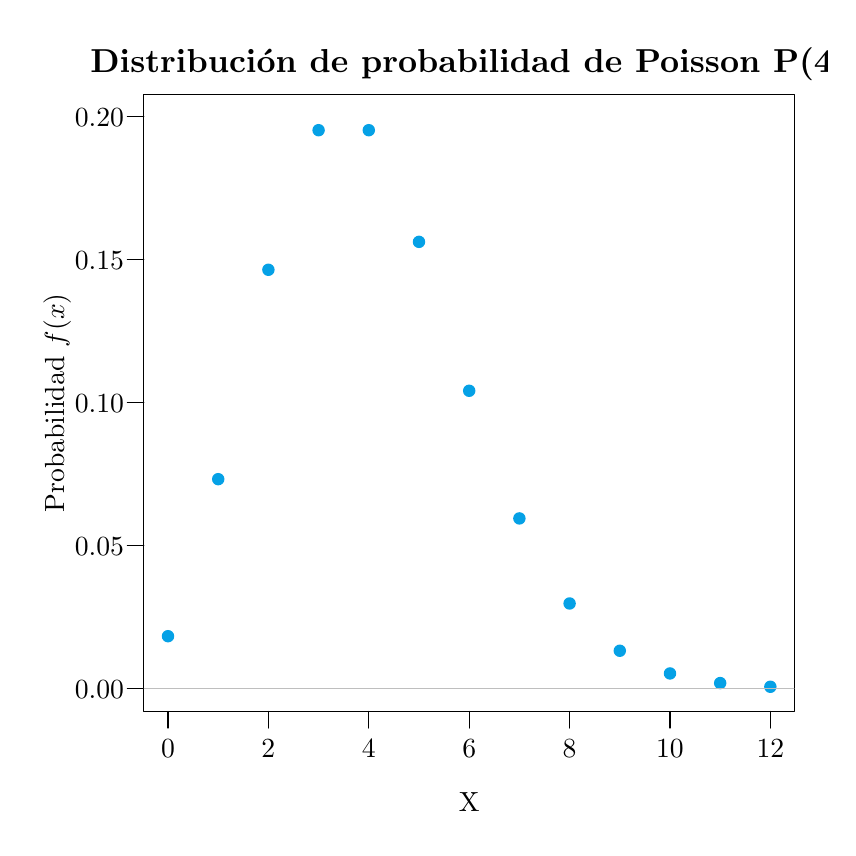
\begin{tikzpicture}[x=1pt,y=1pt]
\definecolor{fillColor}{RGB}{255,255,255}
\path[use as bounding box,fill=fillColor,fill opacity=0.00] (0,0) rectangle (289.08,289.08);
\begin{scope}
\path[clip] ( 42.00, 42.00) rectangle (277.08,265.08);
\definecolor{fillColor}{RGB}{5,161,230}

\path[fill=fillColor] ( 50.71, 69.18) circle (  2.25);

\path[fill=fillColor] ( 68.85,125.93) circle (  2.25);

\path[fill=fillColor] ( 86.98,201.59) circle (  2.25);

\path[fill=fillColor] (105.12,252.03) circle (  2.25);

\path[fill=fillColor] (123.26,252.03) circle (  2.25);

\path[fill=fillColor] (141.40,211.68) circle (  2.25);

\path[fill=fillColor] (159.54,157.87) circle (  2.25);

\path[fill=fillColor] (177.68,111.75) circle (  2.25);

\path[fill=fillColor] (195.82, 81.01) circle (  2.25);

\path[fill=fillColor] (213.96, 63.93) circle (  2.25);

\path[fill=fillColor] (232.10, 55.73) circle (  2.25);

\path[fill=fillColor] (250.23, 52.25) circle (  2.25);

\path[fill=fillColor] (268.37, 50.92) circle (  2.25);
\end{scope}
\begin{scope}
\path[clip] (  0.00,  0.00) rectangle (289.08,289.08);
\definecolor{drawColor}{RGB}{0,0,0}

\path[draw=drawColor,line width= 0.4pt,line join=round,line cap=round] ( 50.71, 42.00) -- (268.37, 42.00);

\path[draw=drawColor,line width= 0.4pt,line join=round,line cap=round] ( 50.71, 42.00) -- ( 50.71, 36.00);

\path[draw=drawColor,line width= 0.4pt,line join=round,line cap=round] ( 86.98, 42.00) -- ( 86.98, 36.00);

\path[draw=drawColor,line width= 0.4pt,line join=round,line cap=round] (123.26, 42.00) -- (123.26, 36.00);

\path[draw=drawColor,line width= 0.4pt,line join=round,line cap=round] (159.54, 42.00) -- (159.54, 36.00);

\path[draw=drawColor,line width= 0.4pt,line join=round,line cap=round] (195.82, 42.00) -- (195.82, 36.00);

\path[draw=drawColor,line width= 0.4pt,line join=round,line cap=round] (232.10, 42.00) -- (232.10, 36.00);

\path[draw=drawColor,line width= 0.4pt,line join=round,line cap=round] (268.37, 42.00) -- (268.37, 36.00);

\node[text=drawColor,anchor=base,inner sep=0pt, outer sep=0pt, scale=  1.00] at ( 50.71, 25.20) {0};

\node[text=drawColor,anchor=base,inner sep=0pt, outer sep=0pt, scale=  1.00] at ( 86.98, 25.20) {2};

\node[text=drawColor,anchor=base,inner sep=0pt, outer sep=0pt, scale=  1.00] at (123.26, 25.20) {4};

\node[text=drawColor,anchor=base,inner sep=0pt, outer sep=0pt, scale=  1.00] at (159.54, 25.20) {6};

\node[text=drawColor,anchor=base,inner sep=0pt, outer sep=0pt, scale=  1.00] at (195.82, 25.20) {8};

\node[text=drawColor,anchor=base,inner sep=0pt, outer sep=0pt, scale=  1.00] at (232.10, 25.20) {10};

\node[text=drawColor,anchor=base,inner sep=0pt, outer sep=0pt, scale=  1.00] at (268.37, 25.20) {12};

\path[draw=drawColor,line width= 0.4pt,line join=round,line cap=round] ( 42.00, 50.26) -- ( 42.00,256.82);

\path[draw=drawColor,line width= 0.4pt,line join=round,line cap=round] ( 42.00, 50.26) -- ( 36.00, 50.26);

\path[draw=drawColor,line width= 0.4pt,line join=round,line cap=round] ( 42.00,101.90) -- ( 36.00,101.90);

\path[draw=drawColor,line width= 0.4pt,line join=round,line cap=round] ( 42.00,153.54) -- ( 36.00,153.54);

\path[draw=drawColor,line width= 0.4pt,line join=round,line cap=round] ( 42.00,205.18) -- ( 36.00,205.18);

\path[draw=drawColor,line width= 0.4pt,line join=round,line cap=round] ( 42.00,256.82) -- ( 36.00,256.82);

\node[text=drawColor,anchor=base east,inner sep=0pt, outer sep=0pt, scale=  1.00] at ( 34.80, 46.82) {0.00};

\node[text=drawColor,anchor=base east,inner sep=0pt, outer sep=0pt, scale=  1.00] at ( 34.80, 98.46) {0.05};

\node[text=drawColor,anchor=base east,inner sep=0pt, outer sep=0pt, scale=  1.00] at ( 34.80,150.10) {0.10};

\node[text=drawColor,anchor=base east,inner sep=0pt, outer sep=0pt, scale=  1.00] at ( 34.80,201.73) {0.15};

\node[text=drawColor,anchor=base east,inner sep=0pt, outer sep=0pt, scale=  1.00] at ( 34.80,253.37) {0.20};

\path[draw=drawColor,line width= 0.4pt,line join=round,line cap=round] ( 42.00, 42.00) --
	(277.08, 42.00) --
	(277.08,265.08) --
	( 42.00,265.08) --
	( 42.00, 42.00);
\end{scope}
\begin{scope}
\path[clip] (  0.00,  0.00) rectangle (289.08,289.08);
\definecolor{drawColor}{RGB}{0,0,0}

\node[text=drawColor,anchor=base,inner sep=0pt, outer sep=0pt, scale=  1.20] at (159.54,272.89) {\bfseries Distribución de probabilidad de Poisson P(4)};

\node[text=drawColor,anchor=base,inner sep=0pt, outer sep=0pt, scale=  1.00] at (159.54,  6.00) {X};

\node[text=drawColor,rotate= 90.00,anchor=base,inner sep=0pt, outer sep=0pt, scale=  1.00] at ( 13.20,153.54) {Probabilidad $f(x)$};
\end{scope}
\begin{scope}
\path[clip] ( 42.00, 42.00) rectangle (277.08,265.08);
\definecolor{drawColor}{RGB}{190,190,190}

\path[draw=drawColor,line width= 0.4pt,line join=round,line cap=round] ( 42.00, 50.26) -- (277.08, 50.26);
\end{scope}
\end{tikzpicture}
}}
  \mode<presentation>{\resizebox{0.55\textwidth}{!}{% Created by tikzDevice version 0.10.1 on 2016-04-19 18:05:49
% !TEX encoding = UTF-8 Unicode
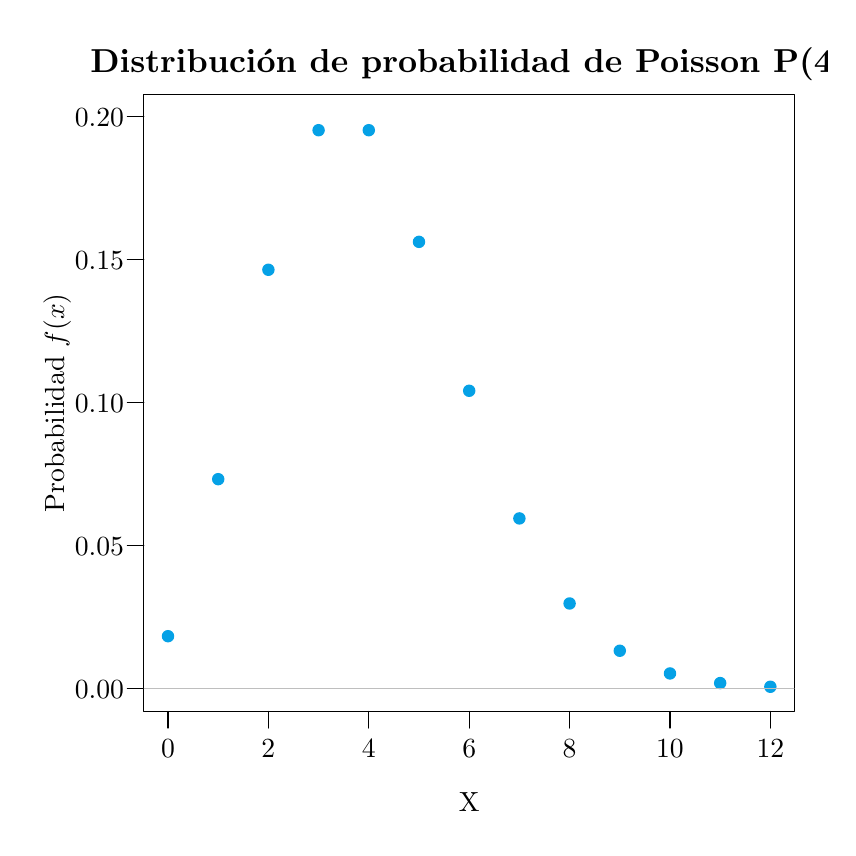
\begin{tikzpicture}[x=1pt,y=1pt]
\definecolor{fillColor}{RGB}{255,255,255}
\path[use as bounding box,fill=fillColor,fill opacity=0.00] (0,0) rectangle (289.08,289.08);
\begin{scope}
\path[clip] ( 42.00, 42.00) rectangle (277.08,265.08);
\definecolor{fillColor}{RGB}{5,161,230}

\path[fill=fillColor] ( 50.71, 69.18) circle (  2.25);

\path[fill=fillColor] ( 68.85,125.93) circle (  2.25);

\path[fill=fillColor] ( 86.98,201.59) circle (  2.25);

\path[fill=fillColor] (105.12,252.03) circle (  2.25);

\path[fill=fillColor] (123.26,252.03) circle (  2.25);

\path[fill=fillColor] (141.40,211.68) circle (  2.25);

\path[fill=fillColor] (159.54,157.87) circle (  2.25);

\path[fill=fillColor] (177.68,111.75) circle (  2.25);

\path[fill=fillColor] (195.82, 81.01) circle (  2.25);

\path[fill=fillColor] (213.96, 63.93) circle (  2.25);

\path[fill=fillColor] (232.10, 55.73) circle (  2.25);

\path[fill=fillColor] (250.23, 52.25) circle (  2.25);

\path[fill=fillColor] (268.37, 50.92) circle (  2.25);
\end{scope}
\begin{scope}
\path[clip] (  0.00,  0.00) rectangle (289.08,289.08);
\definecolor{drawColor}{RGB}{0,0,0}

\path[draw=drawColor,line width= 0.4pt,line join=round,line cap=round] ( 50.71, 42.00) -- (268.37, 42.00);

\path[draw=drawColor,line width= 0.4pt,line join=round,line cap=round] ( 50.71, 42.00) -- ( 50.71, 36.00);

\path[draw=drawColor,line width= 0.4pt,line join=round,line cap=round] ( 86.98, 42.00) -- ( 86.98, 36.00);

\path[draw=drawColor,line width= 0.4pt,line join=round,line cap=round] (123.26, 42.00) -- (123.26, 36.00);

\path[draw=drawColor,line width= 0.4pt,line join=round,line cap=round] (159.54, 42.00) -- (159.54, 36.00);

\path[draw=drawColor,line width= 0.4pt,line join=round,line cap=round] (195.82, 42.00) -- (195.82, 36.00);

\path[draw=drawColor,line width= 0.4pt,line join=round,line cap=round] (232.10, 42.00) -- (232.10, 36.00);

\path[draw=drawColor,line width= 0.4pt,line join=round,line cap=round] (268.37, 42.00) -- (268.37, 36.00);

\node[text=drawColor,anchor=base,inner sep=0pt, outer sep=0pt, scale=  1.00] at ( 50.71, 25.20) {0};

\node[text=drawColor,anchor=base,inner sep=0pt, outer sep=0pt, scale=  1.00] at ( 86.98, 25.20) {2};

\node[text=drawColor,anchor=base,inner sep=0pt, outer sep=0pt, scale=  1.00] at (123.26, 25.20) {4};

\node[text=drawColor,anchor=base,inner sep=0pt, outer sep=0pt, scale=  1.00] at (159.54, 25.20) {6};

\node[text=drawColor,anchor=base,inner sep=0pt, outer sep=0pt, scale=  1.00] at (195.82, 25.20) {8};

\node[text=drawColor,anchor=base,inner sep=0pt, outer sep=0pt, scale=  1.00] at (232.10, 25.20) {10};

\node[text=drawColor,anchor=base,inner sep=0pt, outer sep=0pt, scale=  1.00] at (268.37, 25.20) {12};

\path[draw=drawColor,line width= 0.4pt,line join=round,line cap=round] ( 42.00, 50.26) -- ( 42.00,256.82);

\path[draw=drawColor,line width= 0.4pt,line join=round,line cap=round] ( 42.00, 50.26) -- ( 36.00, 50.26);

\path[draw=drawColor,line width= 0.4pt,line join=round,line cap=round] ( 42.00,101.90) -- ( 36.00,101.90);

\path[draw=drawColor,line width= 0.4pt,line join=round,line cap=round] ( 42.00,153.54) -- ( 36.00,153.54);

\path[draw=drawColor,line width= 0.4pt,line join=round,line cap=round] ( 42.00,205.18) -- ( 36.00,205.18);

\path[draw=drawColor,line width= 0.4pt,line join=round,line cap=round] ( 42.00,256.82) -- ( 36.00,256.82);

\node[text=drawColor,anchor=base east,inner sep=0pt, outer sep=0pt, scale=  1.00] at ( 34.80, 46.82) {0.00};

\node[text=drawColor,anchor=base east,inner sep=0pt, outer sep=0pt, scale=  1.00] at ( 34.80, 98.46) {0.05};

\node[text=drawColor,anchor=base east,inner sep=0pt, outer sep=0pt, scale=  1.00] at ( 34.80,150.10) {0.10};

\node[text=drawColor,anchor=base east,inner sep=0pt, outer sep=0pt, scale=  1.00] at ( 34.80,201.73) {0.15};

\node[text=drawColor,anchor=base east,inner sep=0pt, outer sep=0pt, scale=  1.00] at ( 34.80,253.37) {0.20};

\path[draw=drawColor,line width= 0.4pt,line join=round,line cap=round] ( 42.00, 42.00) --
	(277.08, 42.00) --
	(277.08,265.08) --
	( 42.00,265.08) --
	( 42.00, 42.00);
\end{scope}
\begin{scope}
\path[clip] (  0.00,  0.00) rectangle (289.08,289.08);
\definecolor{drawColor}{RGB}{0,0,0}

\node[text=drawColor,anchor=base,inner sep=0pt, outer sep=0pt, scale=  1.20] at (159.54,272.89) {\bfseries Distribución de probabilidad de Poisson P(4)};

\node[text=drawColor,anchor=base,inner sep=0pt, outer sep=0pt, scale=  1.00] at (159.54,  6.00) {X};

\node[text=drawColor,rotate= 90.00,anchor=base,inner sep=0pt, outer sep=0pt, scale=  1.00] at ( 13.20,153.54) {Probabilidad $f(x)$};
\end{scope}
\begin{scope}
\path[clip] ( 42.00, 42.00) rectangle (277.08,265.08);
\definecolor{drawColor}{RGB}{190,190,190}

\path[draw=drawColor,line width= 0.4pt,line join=round,line cap=round] ( 42.00, 50.26) -- (277.08, 50.26);
\end{scope}
\end{tikzpicture}
}}
  \end{center}

\note{
Sea un hospital en el que se producen por término medio 4 ingresos diarios. Entonces la variable aleatoria $X$ que mide el número de
ingresos en un día sigue un modelo de distribución de Poisson $X\sim P(4)$, y la gráfica de la función de probabilidad es esta. Obsérvese
cómo, aunque teóricamente la variable podría tomar valores hasta $\infty$, la probabilidad de que ocurran más de 10 ingresos ya es casi
despreciable. 
}
\end{frame}


%---------------------------------------------------------------------slide----
\begin{frame}
\frametitle{Distribución de Poisson $P(\lambda)$}
\framesubtitle{Ejemplo del número de nacimientos en una ciudad}
Sea $X\sim P(4)$ la variable que mide el número de ingresos diarios en un hospital. Entonces,
\begin{itemize}
\item La probabilidad de que un día cualquiera se produzcan 5 nacimientos es
\[
f(5) = e^{-4}\frac{4^5}{5!} = 0.1563.
\]
\item La probabilidad de que un día se produzcan menos de 2 nacimientos es
\[
F(1) = f(0)+f(1) = e^{-4}\frac{4^0}{0!} + e^{-4}\frac{4^1}{1!} = 5e^{-4} = 0.0916.
\]
\item La probabilidad de que un día se produzcan más de un 1 nacimiento es
\[
P(X>1) = 1- P(X\leq 1) = 1- F(1) = 1- 0.0916 = 0.9084.
\]
\end{itemize}

\note{
Ya hemos visto que la variable que mide el número de ingresos diarios en un hospital donde por término medio se producen 4 ingresos al día,
sigue un modelo de distribución de Poisson $P(4)$. Entonces:
\begin{itemize}
\item La probabilidad de que un día cualquiera se produzcan 5 ingresos es
\[
f(5) = e^{-4}\frac{4^5}{5!} = 0.1563.
\]
\item La probabilidad de que un día se produzcan menos de 2 ingresos es
\[
F(1) = f(0)+f(1) = e^{-4}\frac{4^0}{0!} + e^{-4}\frac{4^1}{1!} = 5e^{-4} = 0.0916.
\]
\item La probabilidad de que un día se produzcan más de un 1 ingresos es
\[
P(X> 1).
\]
Pero esta probabilidad es $f(1)+f(2)+\cdots$, hasta infinito, de modo que para calcularla tenemos que recurrir a la probabilidad del suceso
contrario, es decir,
\[
P(X> 1) = 1- P(X\leq 1) = 1- F(1) = 1- 0.0916 = 0.9084.
\]
\end{itemize} 
}
\end{frame}


%---------------------------------------------------------------------slide----
\begin{frame}
\frametitle{Aproximación del modelo Binomial mediante el Poisson}
\framesubtitle{Ley de los casos raros}
El modelo de distribución de Poisson surge a partir del modelo de distribución Binomial, cuando el número de repeticiones del ensayo tiende a infinito y la probabilidad de Éxito tiende a cero.

\begin{teorema}[Ley de los casos raros]
La distribución Binomial $X\sim B(n,p)$ tiende a la distribución de Poisson $P(\lambda)$, con $\lambda=n\cdot p$, cuando $n$ tiende a infinito y $p$ tiende a cero, es decir,
\[
  \lim_{n\rightarrow \infty, p\rightarrow 0}\binom{n}{x}p^x(1-p)^{n-x} = e^{-\lambda}\frac{\lambda^x}{x!}.
\]
\end{teorema}

En la práctica, esta aproximación suele utilizarse para $n\geq 30$ y $p\leq 0.1$.

\note{
En realidad, el modelo de distribución de Poisson surge a partir del modelo de distribución Binomial,  cuando el número de ensayos es muy
grande $n\rightarrow \infty$ y la probabilidad de ``éxito'' es muy pequeña $p\rightarrow 0$.

En tales circunstancias, la variable $X\sim B(n,p)$ puede aproximarse mediante el modelo de distribución de Poisson $P(n\cdot p)$.
\[
\lim_{n\rightarrow \infty, p\rightarrow 0}\binom{n}{x}p^x(1-p)^{n-x} = e^{-\lambda}\frac{\lambda^x}{x!}.
\]

En la práctica, esta aproximación suele utilizarse para $n\geq 30$ y $p\leq 0.1$.
}
\end{frame}




%---------------------------------------------------------------------slide----
\begin{frame}
\frametitle{Aproximación del modelo Binomial mediante el Poisson}
\framesubtitle{Ejemplo}
Se sabe que una vacuna produce una reacción adversa en el 4\% de los casos. 
Si se vacunan una muestra 50 personas, ¿cuál es la probabilidad de que haya
más de 2 personas con reacción adversa?

La variable que mide el número de personas con reacción adversa en la muestra sigue un modelo de distribución binomial $X\sim B(50,\,0.04)$, pero como $n=50>30$ y $p=0.04<0.1$, se cumplen las condiciones de la ley de los casos raros y se utilizar la distribución de Poisson $P(50\cdot 0.04)=P(2)$ para realizar los cálculos.

\begin{align*}
P(X>2) &= 1 -P(X\leq 2) = 1-f(0)-f(1)-f(2) = 1-e^{-2}\frac{2^0}{0!}-e^{-2}\frac{2^1}{1!}-e^{-2}\frac{2^2}{2!} =\\
&= 1-5e^{-2} = 0.3233.
\end{align*}

\note{
Veamos un ejemplo de cúando aplicar la ley de los casos raros. 

Se sabe que una vacuna produce una reacción adversa en el 4\% de los casos. Si se vacunan 50 personas, ¿cuál es la probabilidad de que haya
más de 2 personas con reacción adversa?

Está claro que la variable que mide el número de personas con reacción adversa entre las 50 personas vacunadas sigue un modelo de
distribución binomial $X\sim B(50,\,0.04)$, pero como $n=50>30$ y $p=0.04<0.1$, se cumplen las condiciones de la ley de los casos raros y se
puede aproximar mediante una distribución de Poisson $P(50\cdot 0.04)=P(2)$.

Así pues, utilizando la fórmula de la función de probabilidad de la distribución de Poisson, se tiene
\begin{align*}
P(X>2) &= 1 -P(X\leq 2) = 1-f(0)-f(1)-f(2) = 1-e^{-2}\frac{2^0}{0!}-e^{-2}\frac{2^1}{1!}-e^{-2}\frac{2^2}{2!} =\\
&= 1-5e^{-2} = 0.3233.
\end{align*}
}
\end{frame}
